\chapter{Chapter I}
\section{Pengenalan Python}
Python adalah Bahasa pemrograman interpretatif (dalam ilmu komputer penerjemah) multiguna dengan filosopi perancangan yang berfokus pada tingkat keterbacaan kode. Python merupakan bahasa pemrograman yang mudah dibaca dan dapat digunakan untuk berbagai macam proyek. Python diklaim sebagai bahasa yang menggabungkan kapabilitas, kemampuan, dengan sintaksis kode yang sangat jelas, dan dilengkapi dengan fungsionalitas pustaka standar yang besar serta komprehensif.Python dikembangkan oleh Guido van Rossum pada tahun 1990 di Stichting Mathematisch Centrum (CWI), Amsterdam sebagai kelanjutan dari bahasa pemrograman ABC. Versi terakhir yang dikeluarkan CWI adalah 1.2.Tahun 1995, Guido pindah ke CNRI di Virginia Amerika sambil terus melanjutkan pengembangan Python. Versi terakhir yang dikeluarkan adalah 1.6. Tahun 2000, Guido dan para pengembang inti Python pindah ke BeOpen.com yang merupakan sebuah perusahaan komersial dan membentuk BeOpen PythonLabs. Python 2.0 dikeluarkan oleh BeOpen. Setelah mengeluarkan Python 2.0, Guido dan beberapa anggota tim PythonLabs pindah ke DigitalCreations

Saat ini pengembangan Python terus dilakukan oleh sekumpulan pemrogram yang dikoordinir Guido dan Python Software Foundation. Python Software Foundation adalah sebuah organisasi non-profit yang dibentuk sebagai pemegang hak cipta intelektual Python sejak versi 2.1 dan dengan demikian mencegah Python dimiliki oleh perusahaan komersial. Saat ini distribusi Python sudah mencapai versi 2.7.14 dan versi 3.6.3
Nama Python dipilih oleh Guido sebagai nama bahasa ciptaannya karena kecintaan Guido pada acara televisi Monty Python's Flying Circus. Oleh karena itu seringkali ungkapan-ungkapan khas dari acara tersebut seringkali muncul dalam korespondensi antar pengguna Python. Python memiliki beberapa versi mulai dari versi yang Python 1.0 bulan Januari 1994 sampai yang terbaru Python 3.7 bulan 27 Juni 2018.

Versi python yang 2.0 berbeda dengan python yang 3.0. Beberapa perbedaannya yaitu:

\begin{enumerate}
\item \textbf{Syntax untuk mencetak teks atau yang lainnya}.\\
Pada python 2 syntaxnya yaitu: bisa menggunakan tanda kurung atau tidak. Sedangkan pada python 3 syntaxnya harus menggunakan tanda kurung, jika tidak maka syntaxnya akan error. Contoh:\\
\begin{itemize}
\item Pada python 2, syntax:
\end{itemize}
        print “tidak pakek kurung bisa”\\
        Print(”pakek kurung juga bisa”)\\
        Print”ini”,;print”mencetak satu baris”\\
        Hasil :    \\

	\begin{figure}[h]
	\centering
	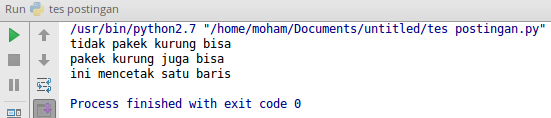
\includegraphics[width=10cm]{gambar/satu.png}
	\caption{hasil gambar python 2}
	\label{fig:gambar}
	\end{figure}
	\begin{itemize}
	\item Pada python 3, syntax:
		print(“harus pakai kurung”)\\
		print(“ini digunakan untuk”, end=””)\\
		print(“python”)\\
		Hasil:\\
		
\begin{figure}[!htbp]
\centering
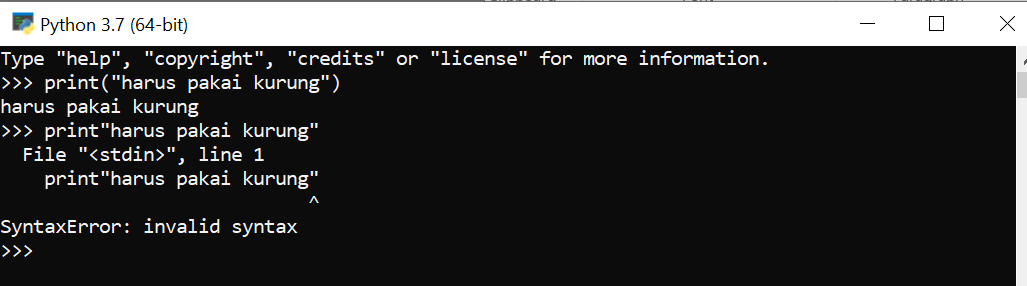
\includegraphics[width=10cm]{gambar/dua.png}
\caption{hasil gambar python 3}
\end{figure}
\end{itemize}
\item \textbf{Syntax untuk meminta inputan}\\
Pada python 2 jika ingin meminta inputan kita harus menggunakan syntax seperti yang ada di bawah .
Sedangkan pada python 3 kita hanya memerlukn syntax dibawah. Contoh:
\begin{itemize}
\item Pada python 2, syntax:\\
			nama = raw-input(‘masukkan nama anda :’)\\
			print nama\\
			Catatan: garis penghubung di atas di ubah menjadi garis bawah.\\
			Hasil:\\
\begin{figure}[!htbp]
\centering
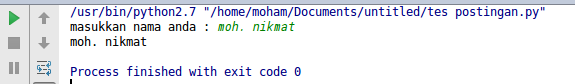
\includegraphics[width=10cm]{gambar/tiga.png}
\caption{hasil gambar python 2}
\end{figure}
\item Pada python 3, syntax:
			nama = input(“masukkan nama anda: ”)\\
			print(nama)\\Hasil:\\
\begin{figure}[!htbp]
\centering
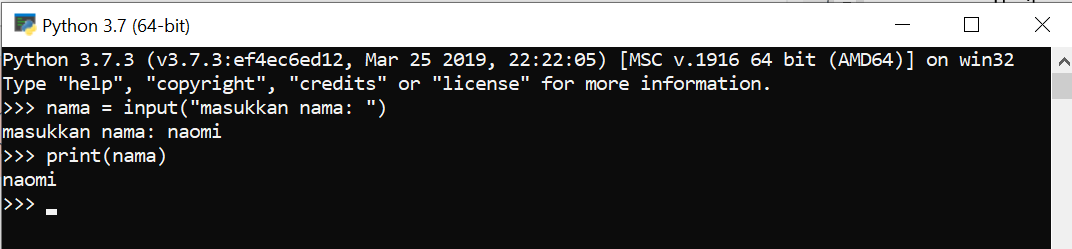
\includegraphics[width=10cm]{gambar/empat.png}
\caption{hasil gambar python 3}
\end{figure}
\end{itemize}
\item Hasil Operator Pembagian\\Pada python 2 hasil pembagian 3/2 adalah 1. Sedangkan pada python 3 yaitu 1,5. Contoh:
\begin{itemize}
\item Pada python 2
			print“3/2=”, 3/2\\
			print“3//2=”, 3//2\\
			print“3/2.0=”, 3/2.0\\
			print“3//2.0=”, 3//2.0\\Hasil:\\
\begin{figure}[!htbp]
\centering
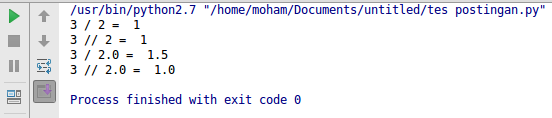
\includegraphics[width=10cm]{gambar/lima.png}
\caption{hasil gambar python 2}
\end{figure}
\item Pada python 2
			print“3/2=”, 3/2\\
			print“3//2=”, 3//2\\
			print“3/2.0=”, 3/2.0\\
			print“3//2.0=”, 3//2.0\\Hasil:\\
\begin{figure}[!htbp]
\centering
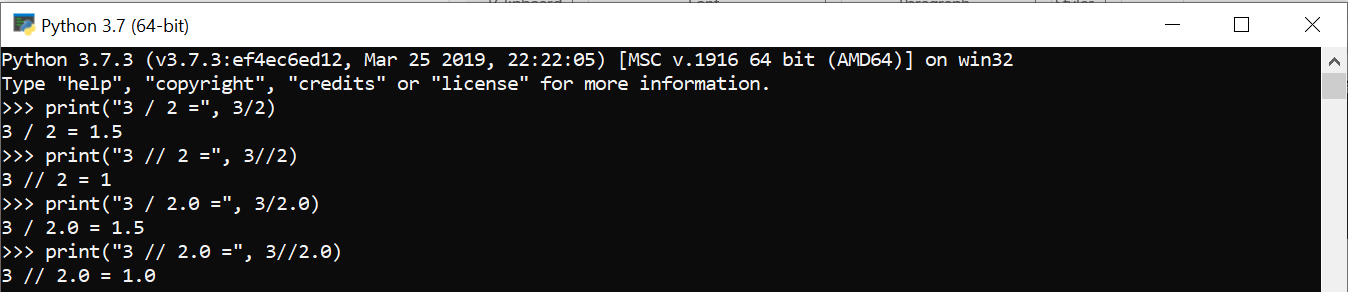
\includegraphics[width=10cm]{gambar/enam.png}
\caption{hasil gambar python 3}
\end{figure}
\end{itemize}
\end{enumerate}

\section{Python dalam Dunia Pekerjaan}
Python dapat digunakan untuk berbagai  pengembangan perangkat lunak dan dapat berjalan di berbagai platform sistem operasi. Maka dari itu Bahasa pemrograman python sangat dibutuhkan dalam dunia pekerjaan. Python sebenarnya masih jarang di Indonesia, dan itu bukan berarti Bahasa pemrograman python lemah. Sebenarnya python lebih banyak di cari di level internasional. Implementasi dan penggunaan python pada dunia pekerjaan yaitu karena python dikenal memiliki banyak kelebihan, dan manfaat yaitu untuk pengembangan web, video game, GUI desktop, hingga perangkat lunak. Dan hal- hal itulah yang paling sering dan banyak di jumpai pada dunia pekerjaan.

\section{Instalisasi}
\begin{enumerate}
\item Install Python
\begin{itemize}
\item Buka link https://www.python.org/downloads/release/python-380/
\item Kemudian download python 3.
\begin{figure}[!htbp]
\centering
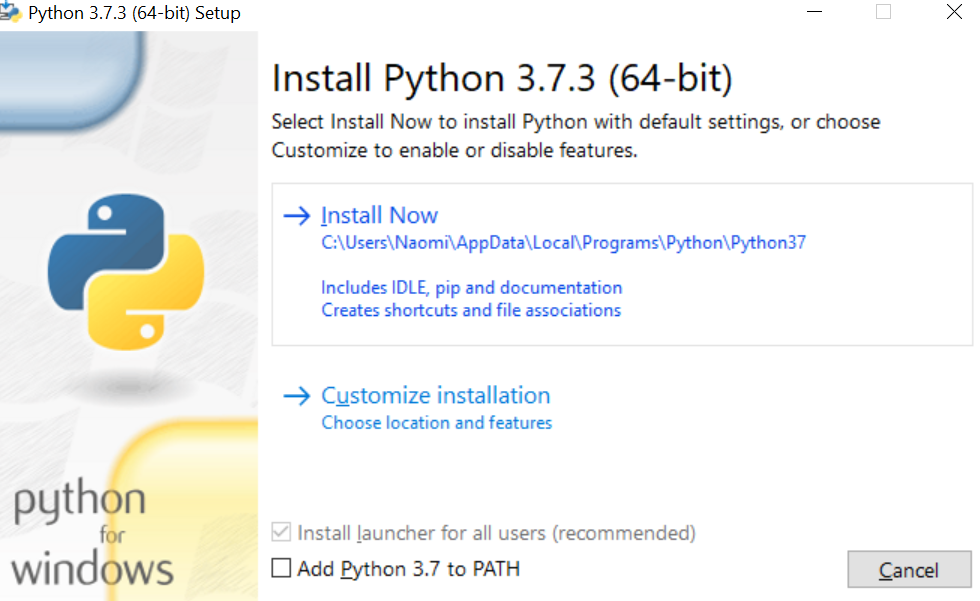
\includegraphics[width=10cm]{gambar/py1.png}
\caption{install python 3}
\end{figure}
\item Kemudian klik “Install Now”.
\begin{figure}[!htbp]
\centering
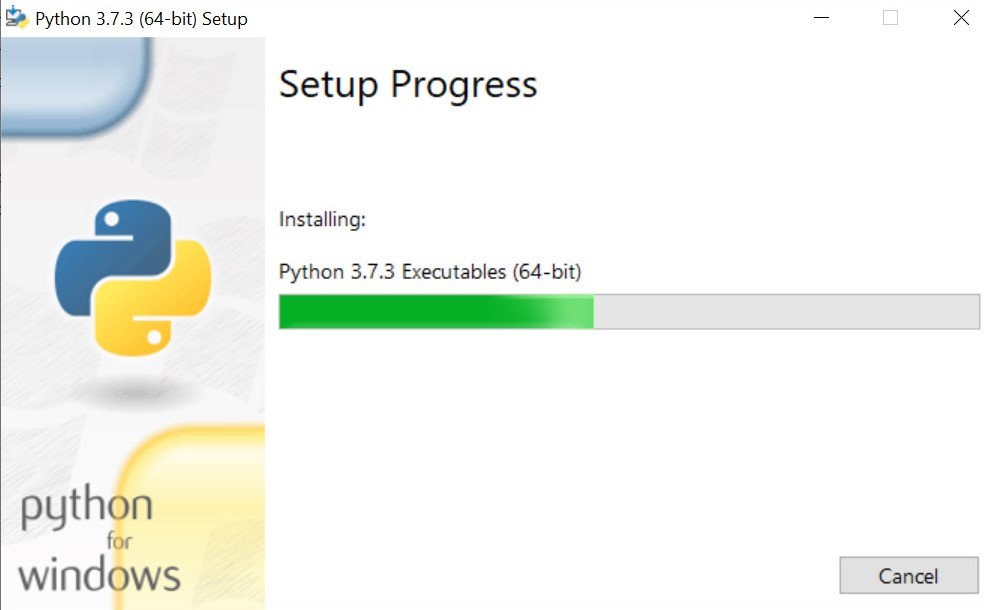
\includegraphics[width=10cm]{gambar/py2.jpg}
\caption{install python 3}
\end{figure}
\item Lalu tunggu instalisasi sampai selesai.
\begin{figure}[!htbp]
\centering
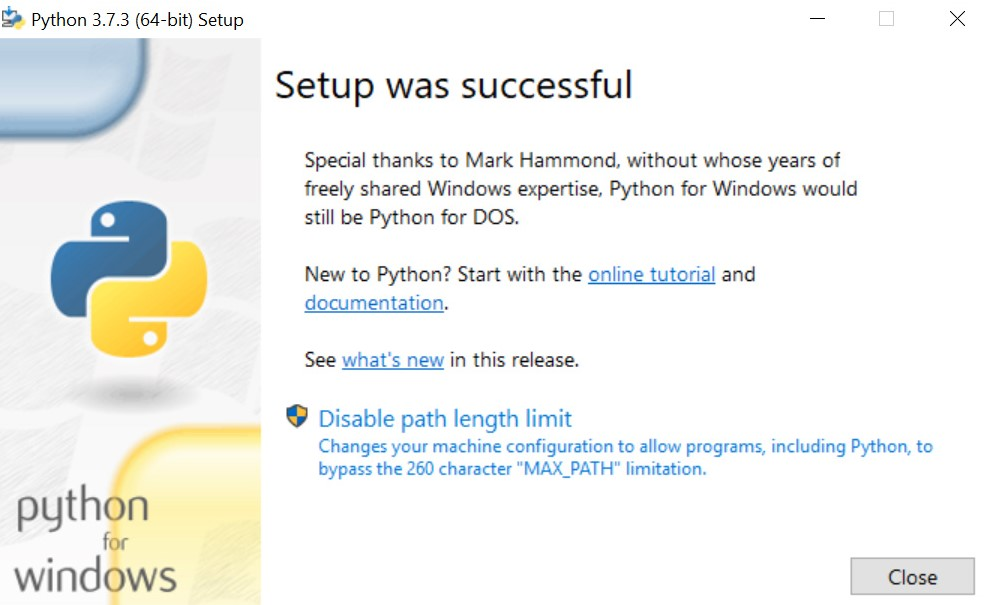
\includegraphics[width=10cm]{gambar/py3.jpg}
\caption{install python 3}
\end{figure}
\item Jika sudah selesai maka akan muncul seperti gambar di atas, yang artinya python sudah terinstal.
\end{itemize}
\item Instal pip
\begin{itemize}
\item Buka CDM(Command Prompt) melalui Start atau dengan cara tekan Windows+R secara bersamaan di keyboard.
\begin{figure}[!htbp]
\centering
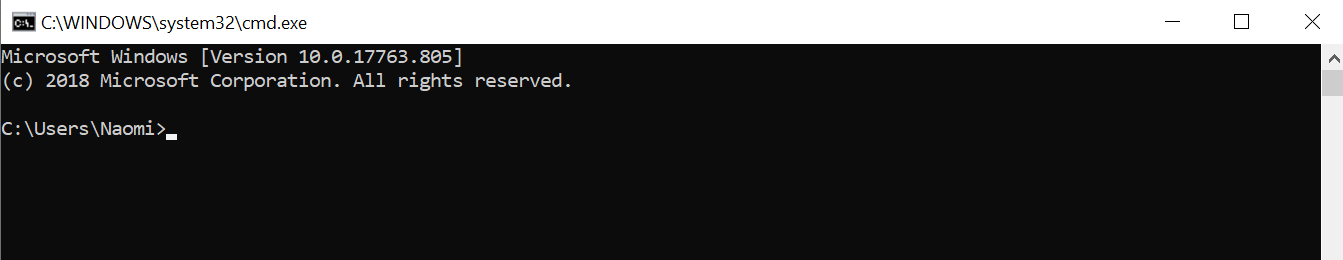
\includegraphics[width=10cm]{gambar/pip0.png}
\caption{install pip}
\end{figure}
\item Kemudian ketik “pip --version” pada CMD, lalu enter. Maka akan muncul seperti pada gambar.
\begin{figure}[!htbp]
\centering
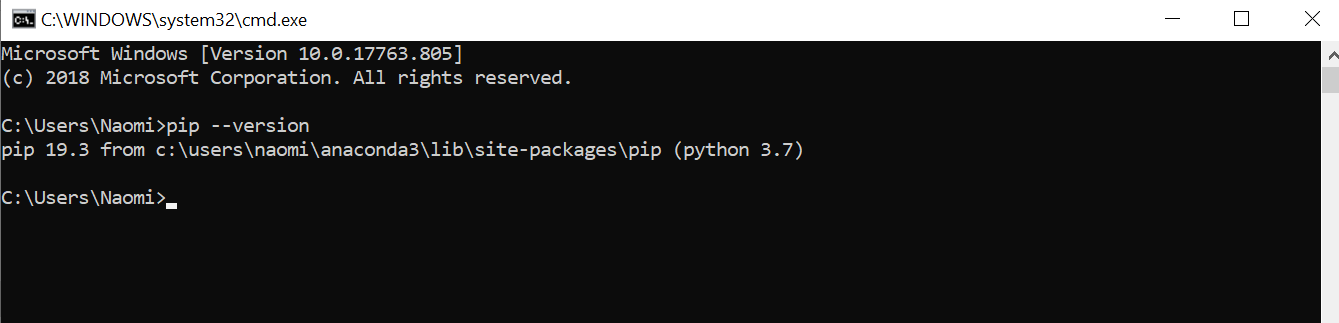
\includegraphics[width=10cm]{gambar/pip1.png}
\caption{install pip}
\end{figure}
\item Lalu ketik “python –m pip install –U pip” sepeti pada gambar.
\begin{figure}[!htbp]
\centering
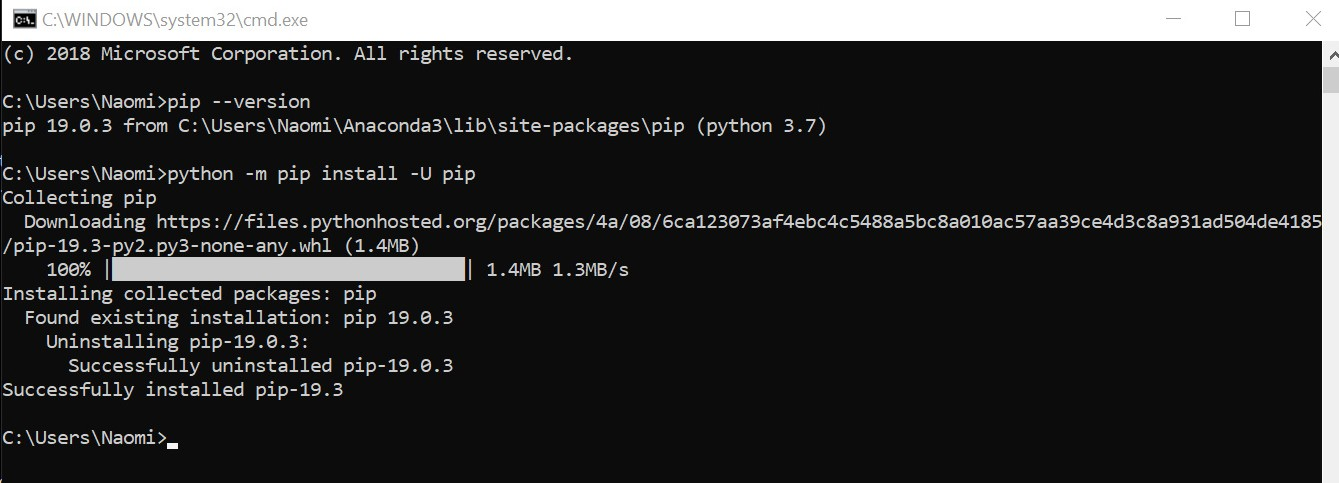
\includegraphics[width=10cm]{gambar/pip2.jpg}
\caption{install pip}
\end{figure}
\item Pip install python selesai.
\end{itemize}
\item Cara Setting Environment
\begin{itemize}
\item Pertama tama buka Anaconda Navigator.
\begin{figure}[!htbp]
\centering
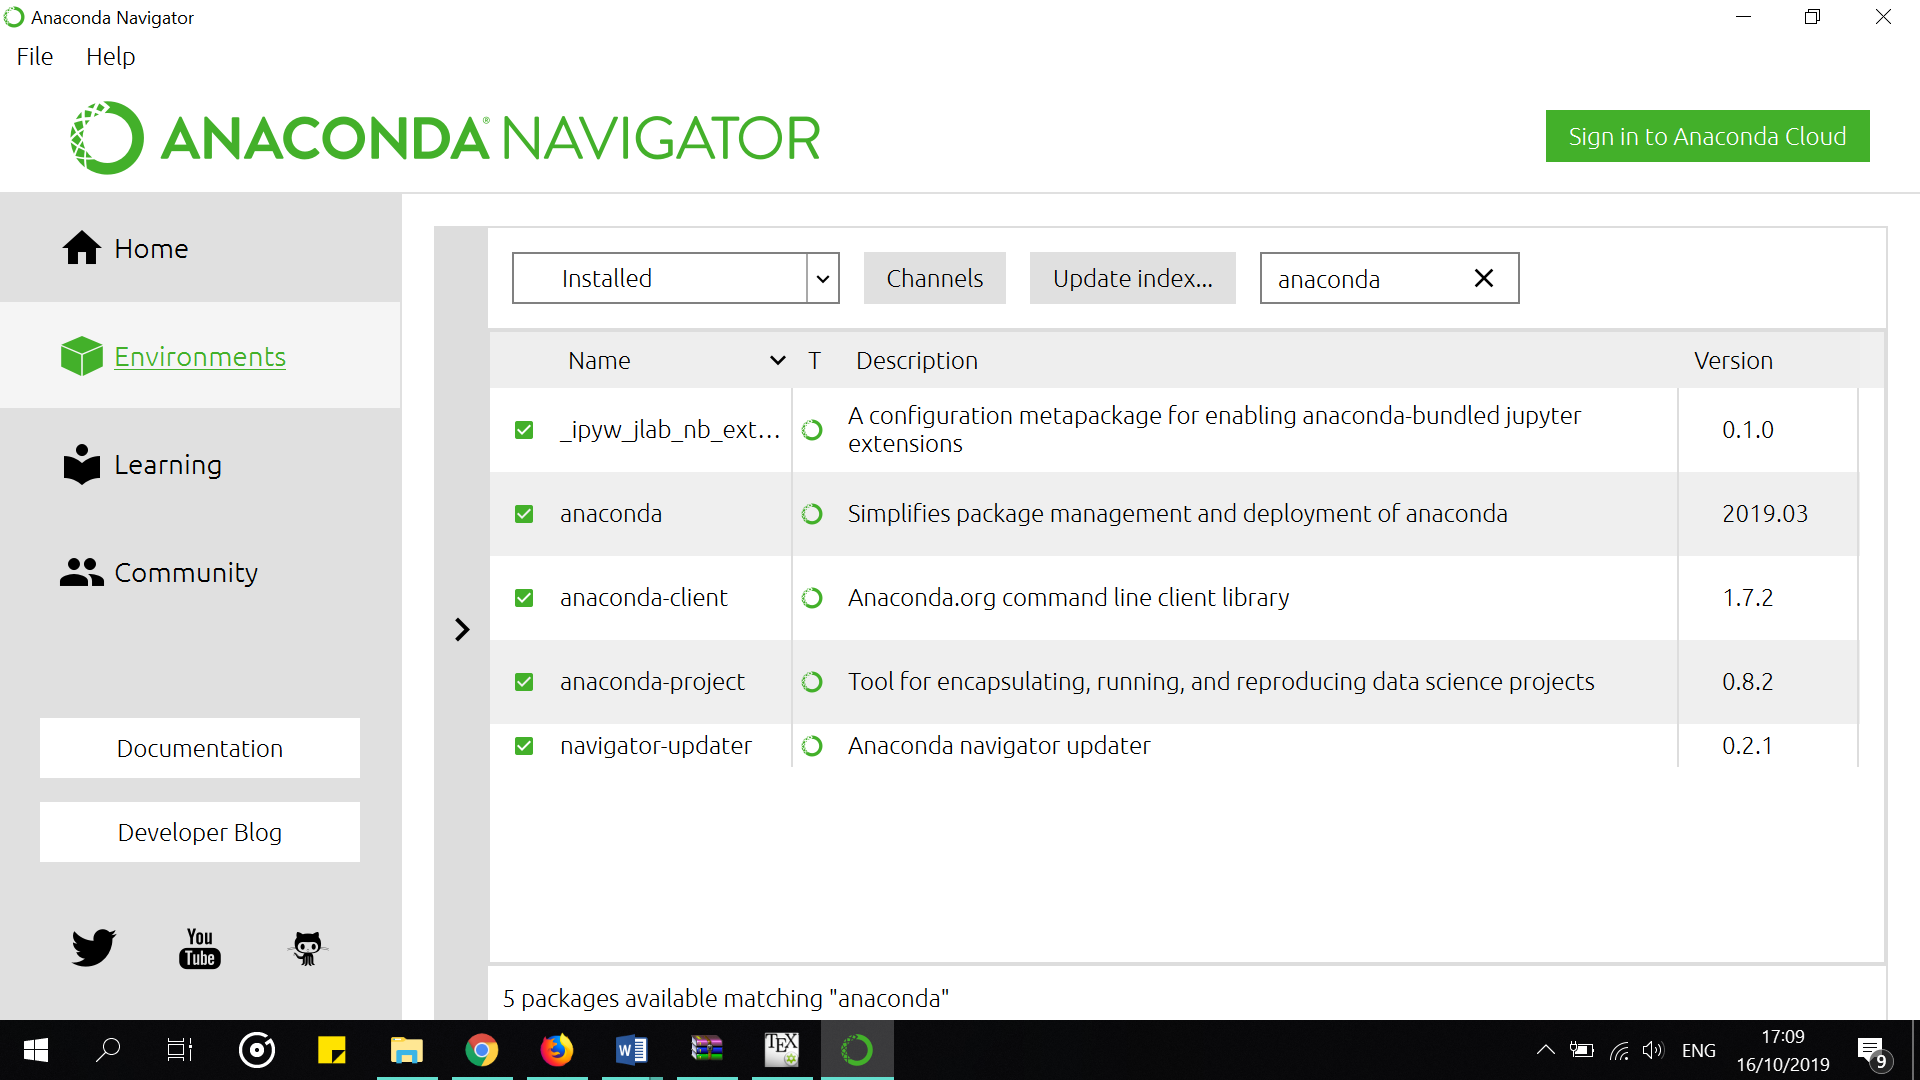
\includegraphics[width=10cm]{gambar/envi3.png}
\caption{environment}
\end{figure}
\item Lalu klik Environment
\begin{figure}[!htbp]
\centering
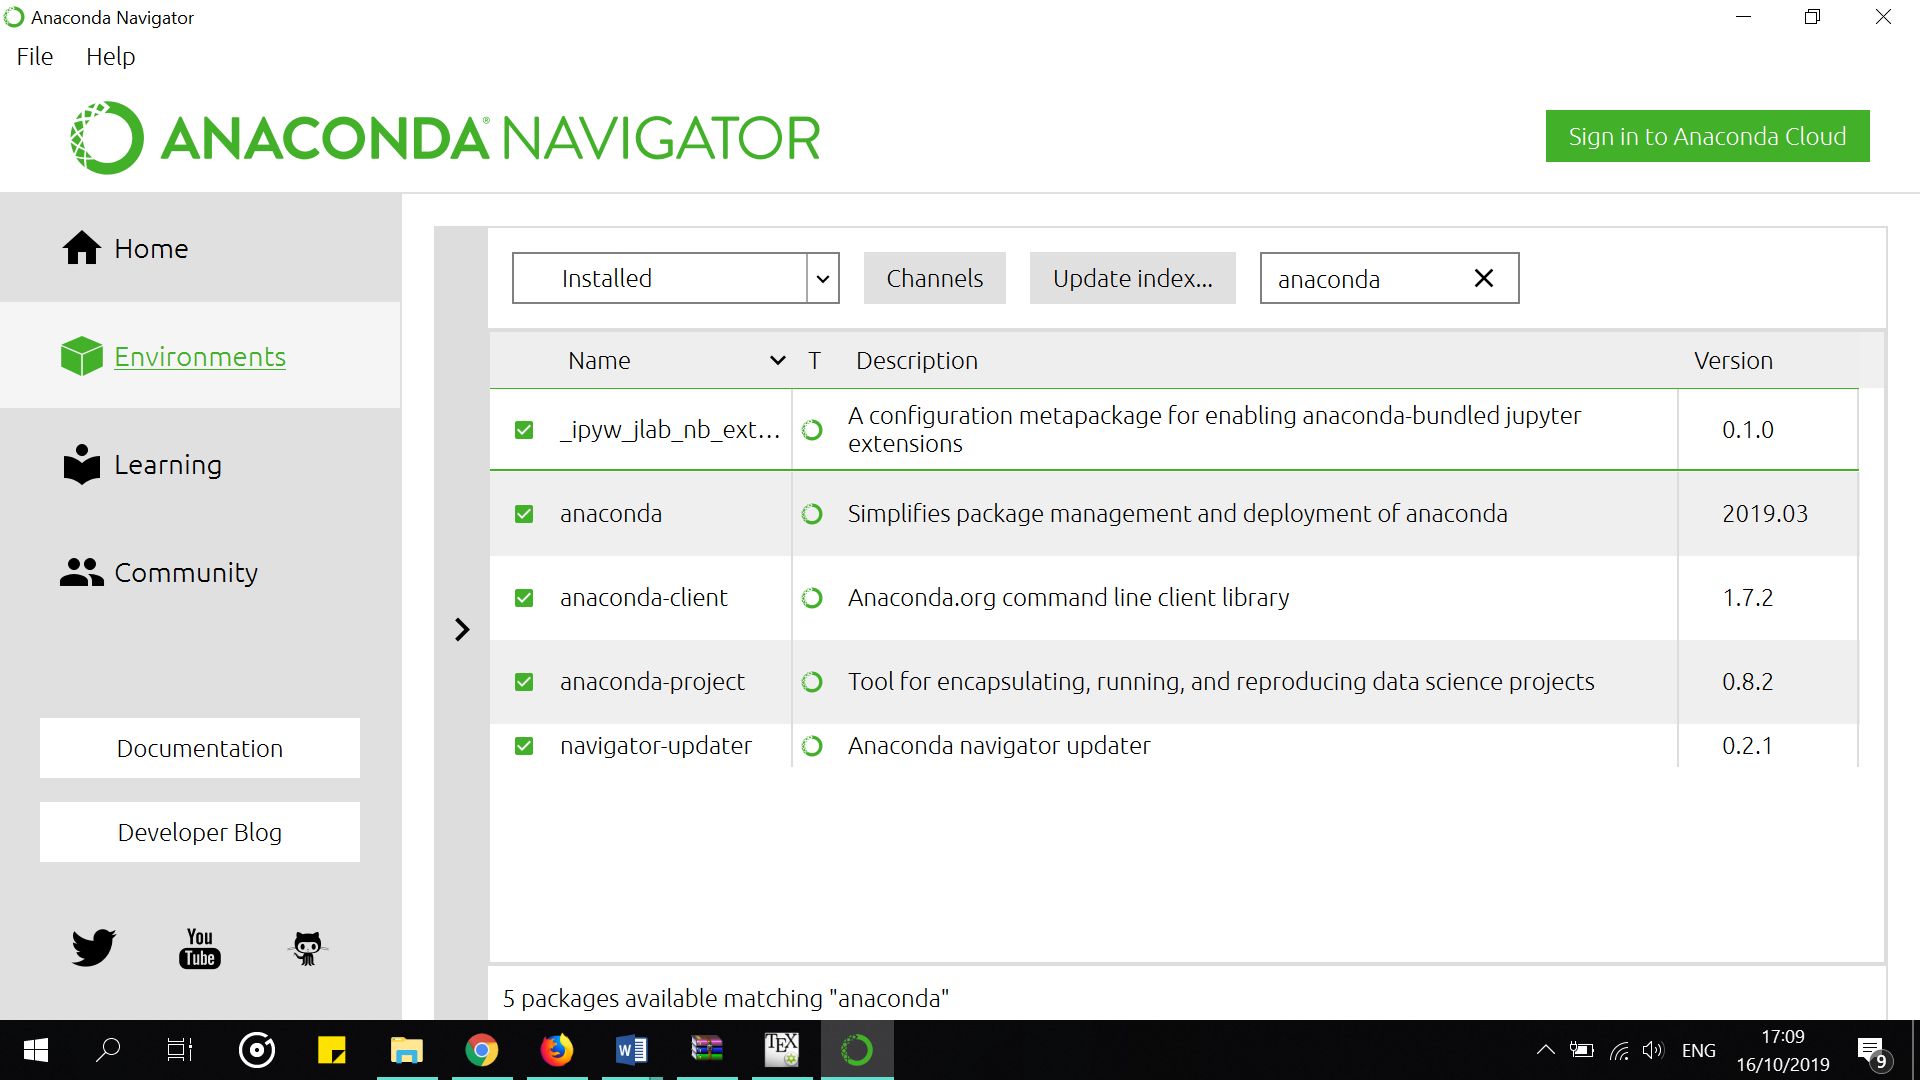
\includegraphics[width=10cm]{gambar/envi4.png}
\caption{environment}
\end{figure}
\item lalu klik centang hijau yang ada di sebelah kiri. seperti berikut
\begin{figure}[!htbp]
\centering
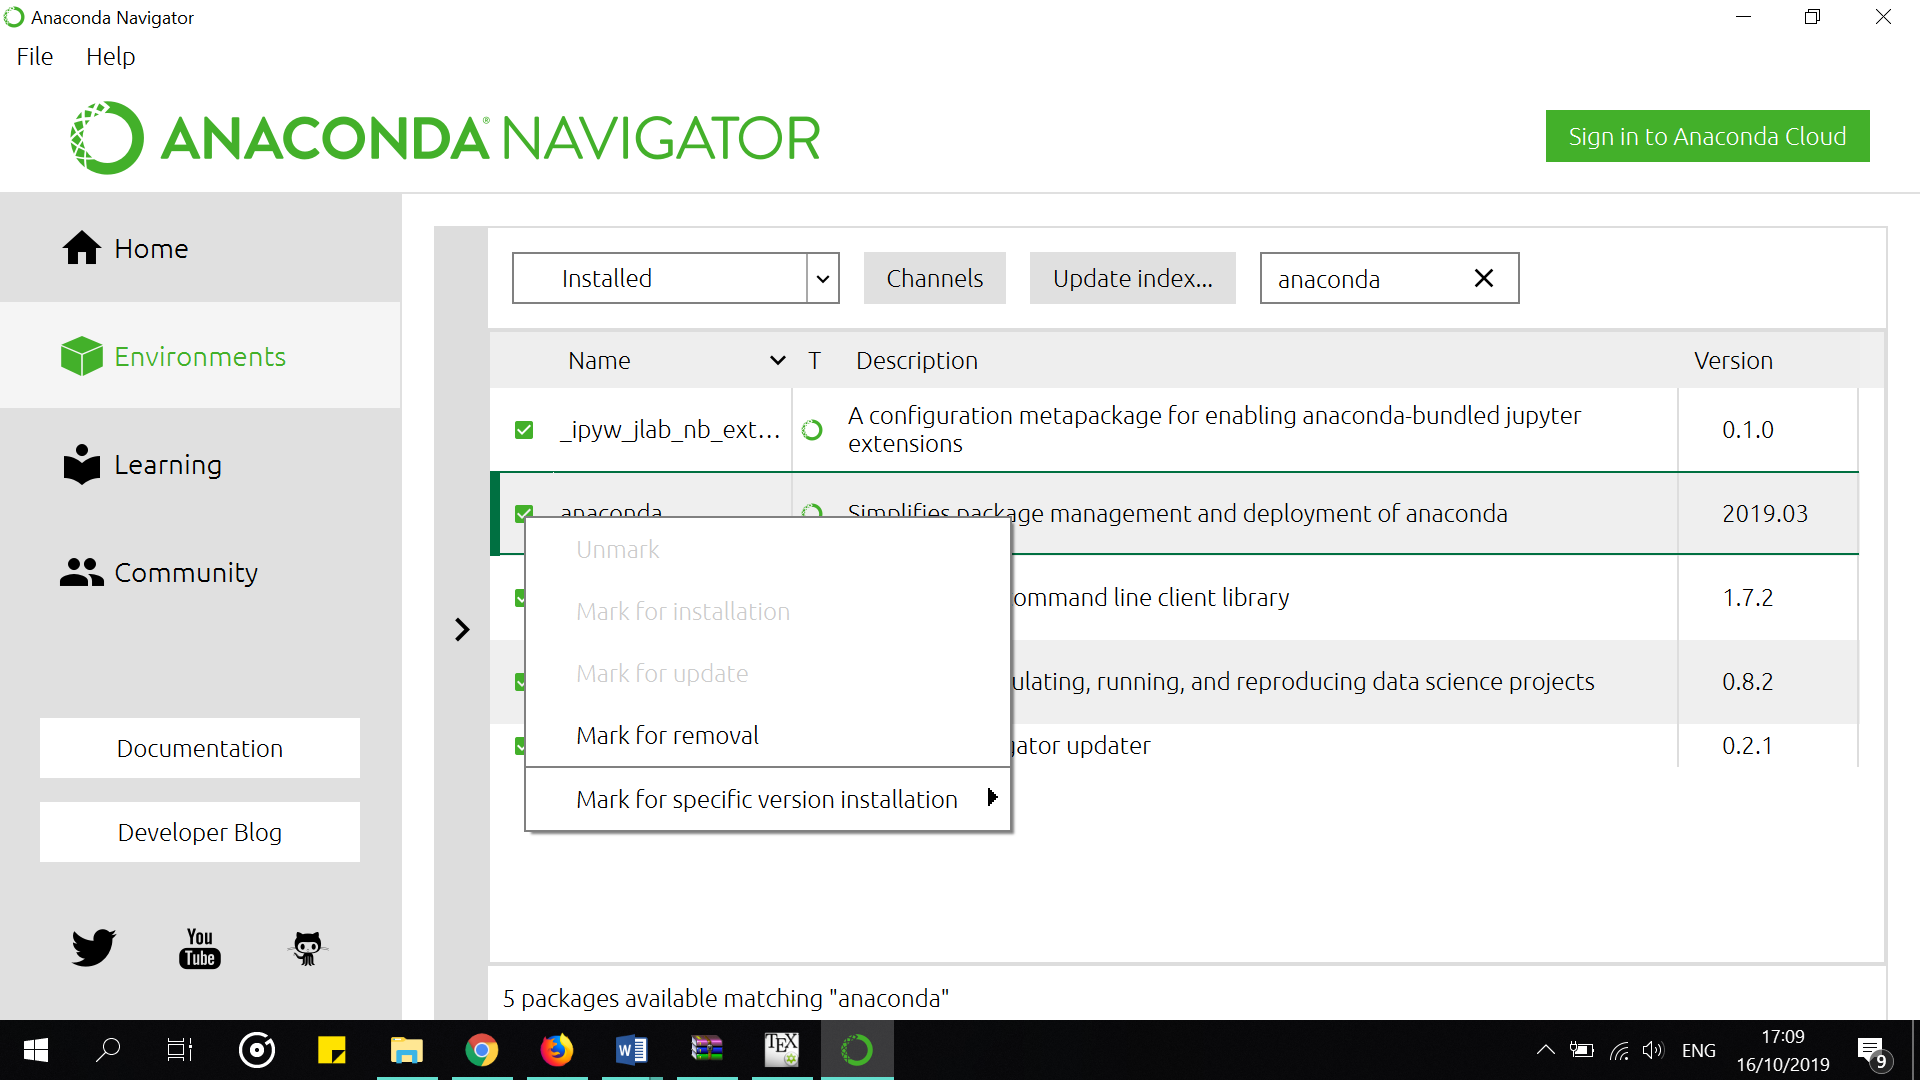
\includegraphics[width=10cm]{gambar/envi5.png}
\caption{environment}
\end{figure}
\item Arahkan pointer ke bagian yang paling bawah
\begin{figure}[!htbp]
\centering
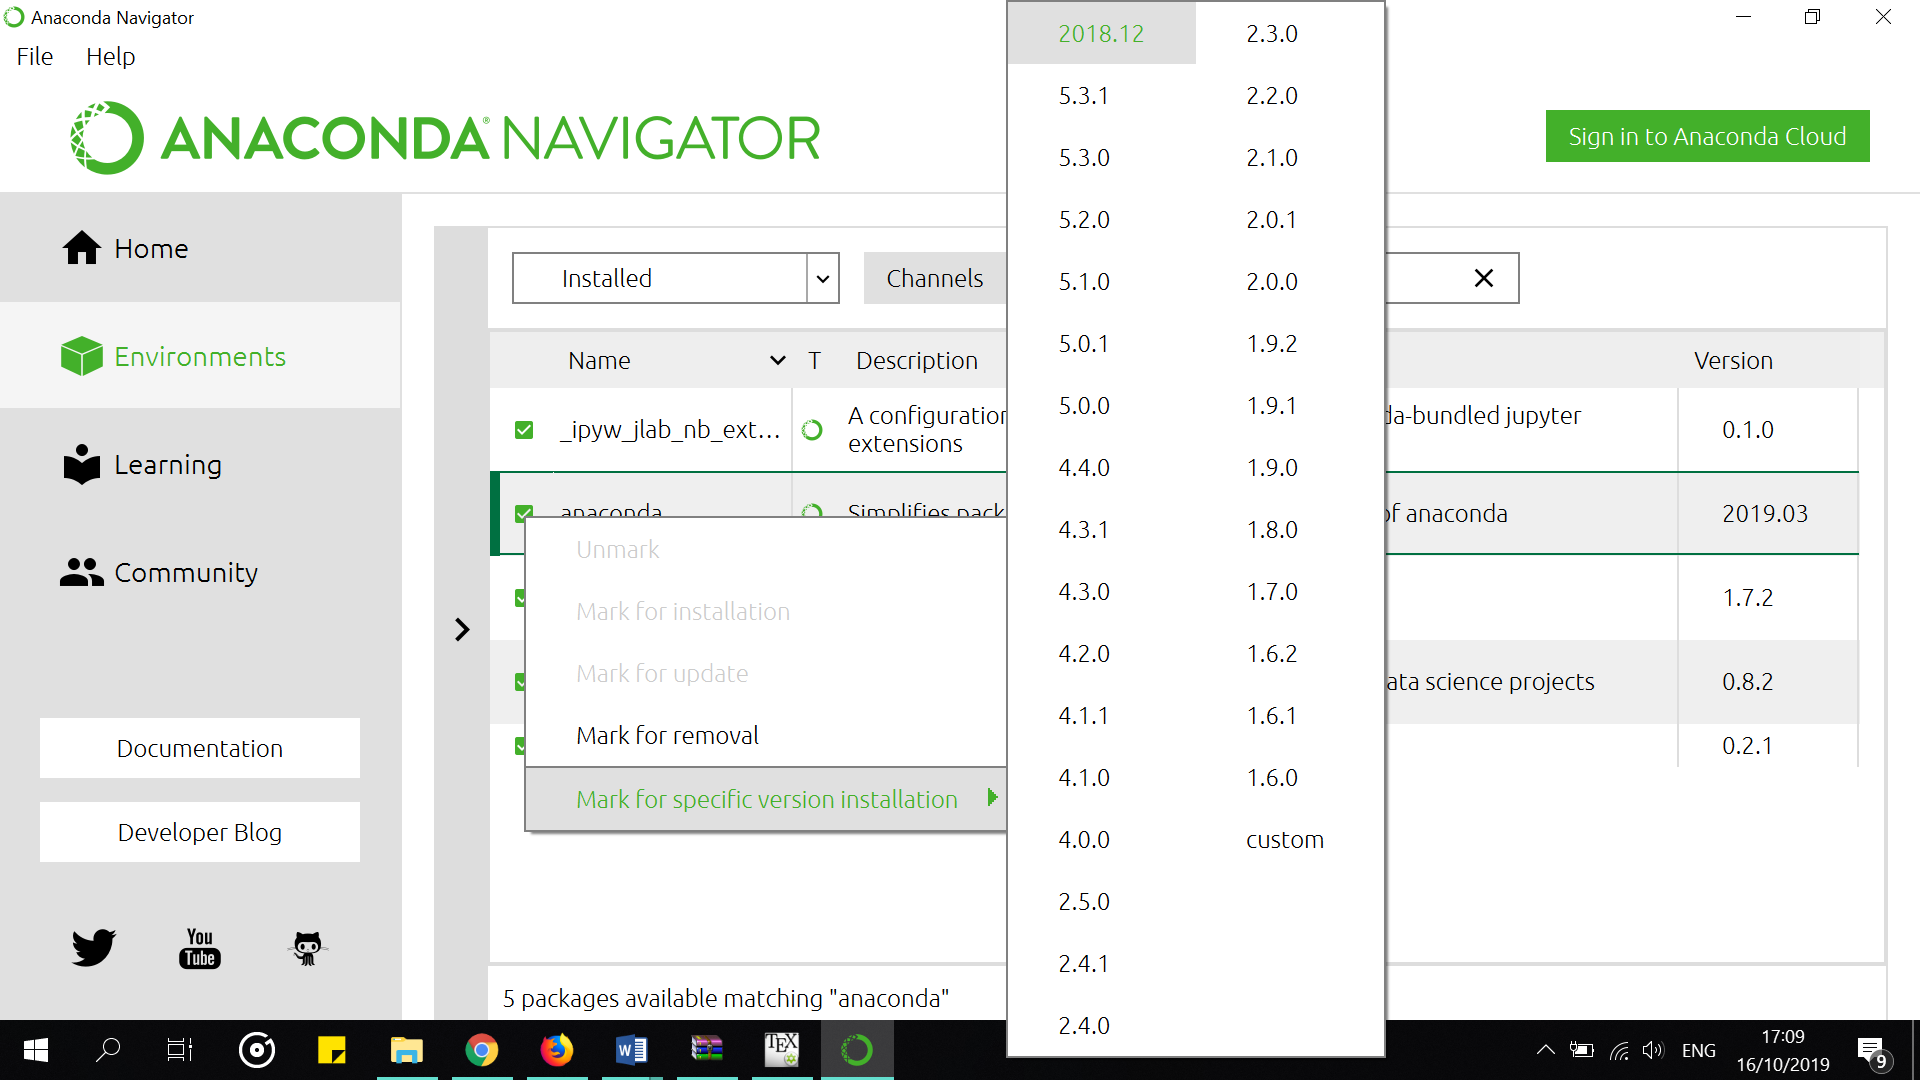
\includegraphics[width=10cm]{gambar/envi6.png}
\caption{environment}
\end{figure}
\item Lalu klik versi yang paling terbaru.
\begin{figure}[!htbp]
\centering
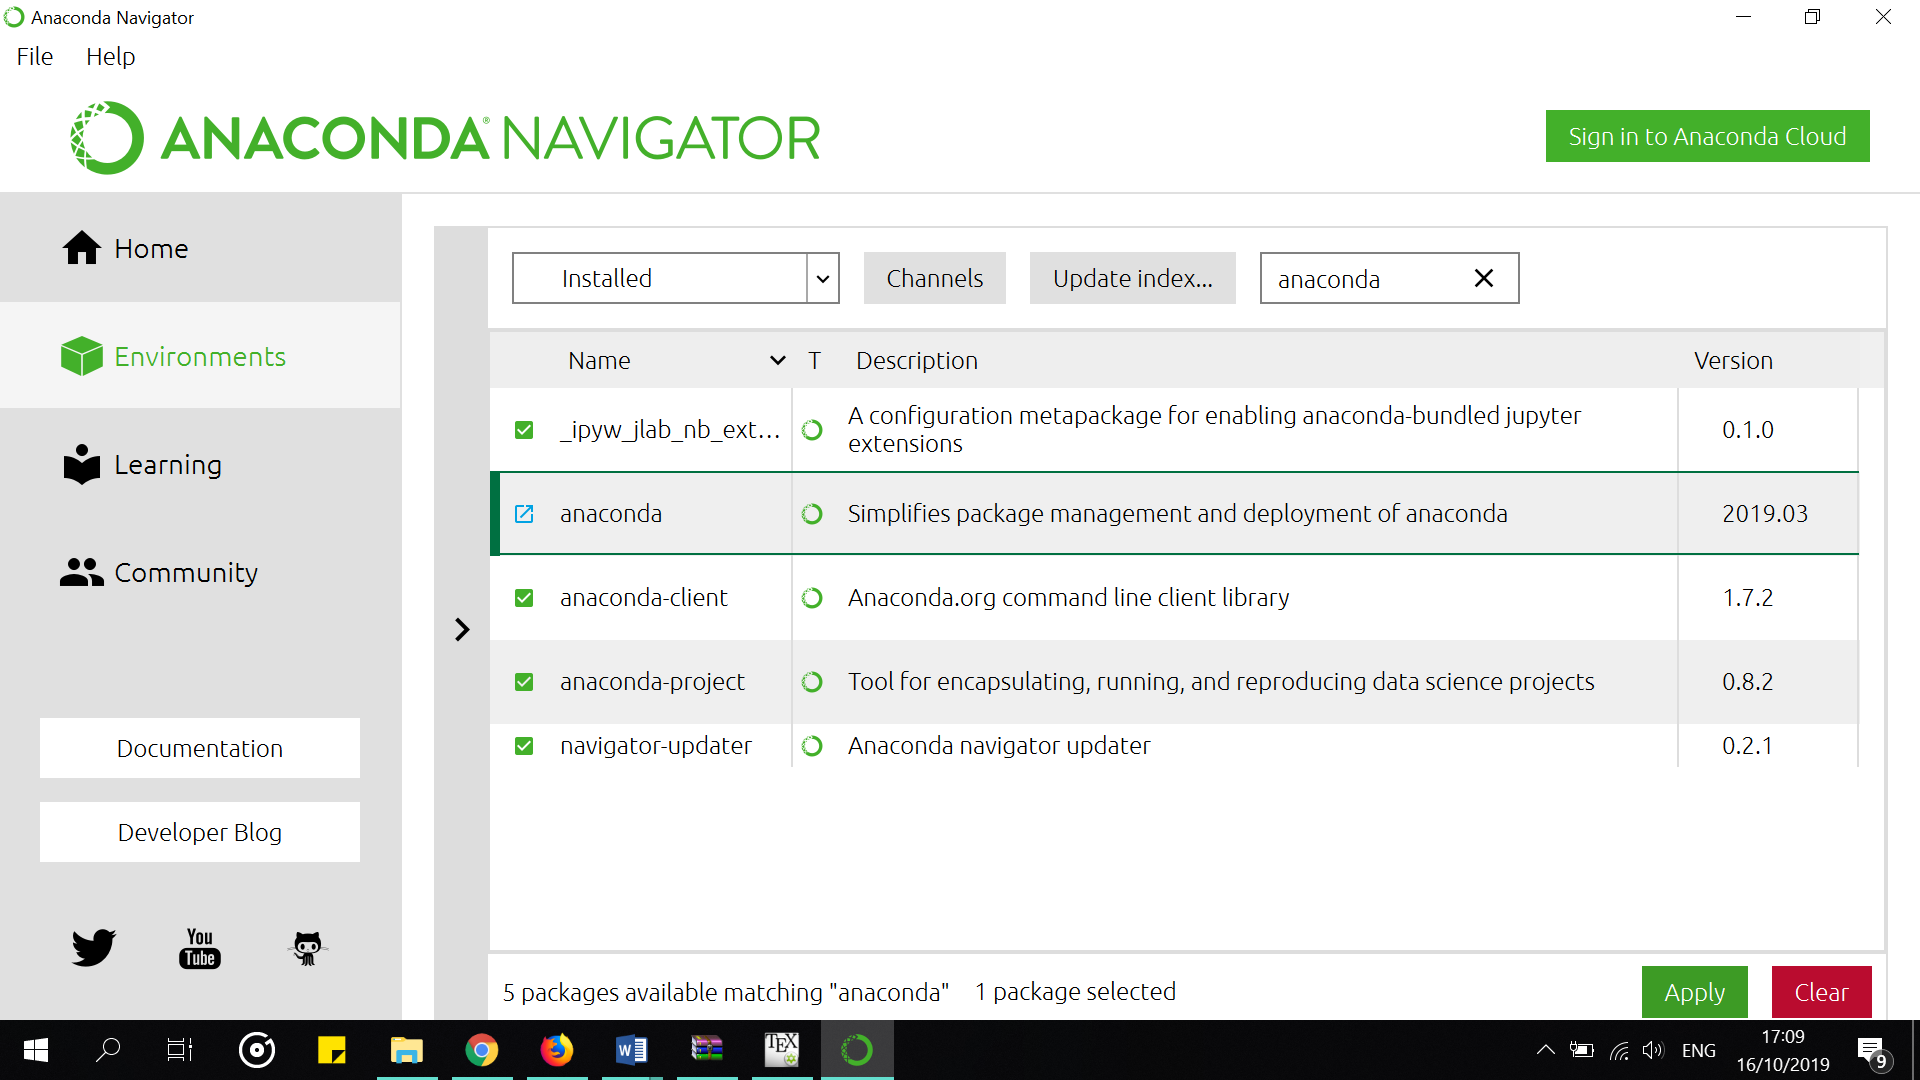
\includegraphics[width=10cm]{gambar/envi7.png}
\caption{environment}
\end{figure}
\item Kemudian Apply.
\begin{figure}[!htbp]
\centering
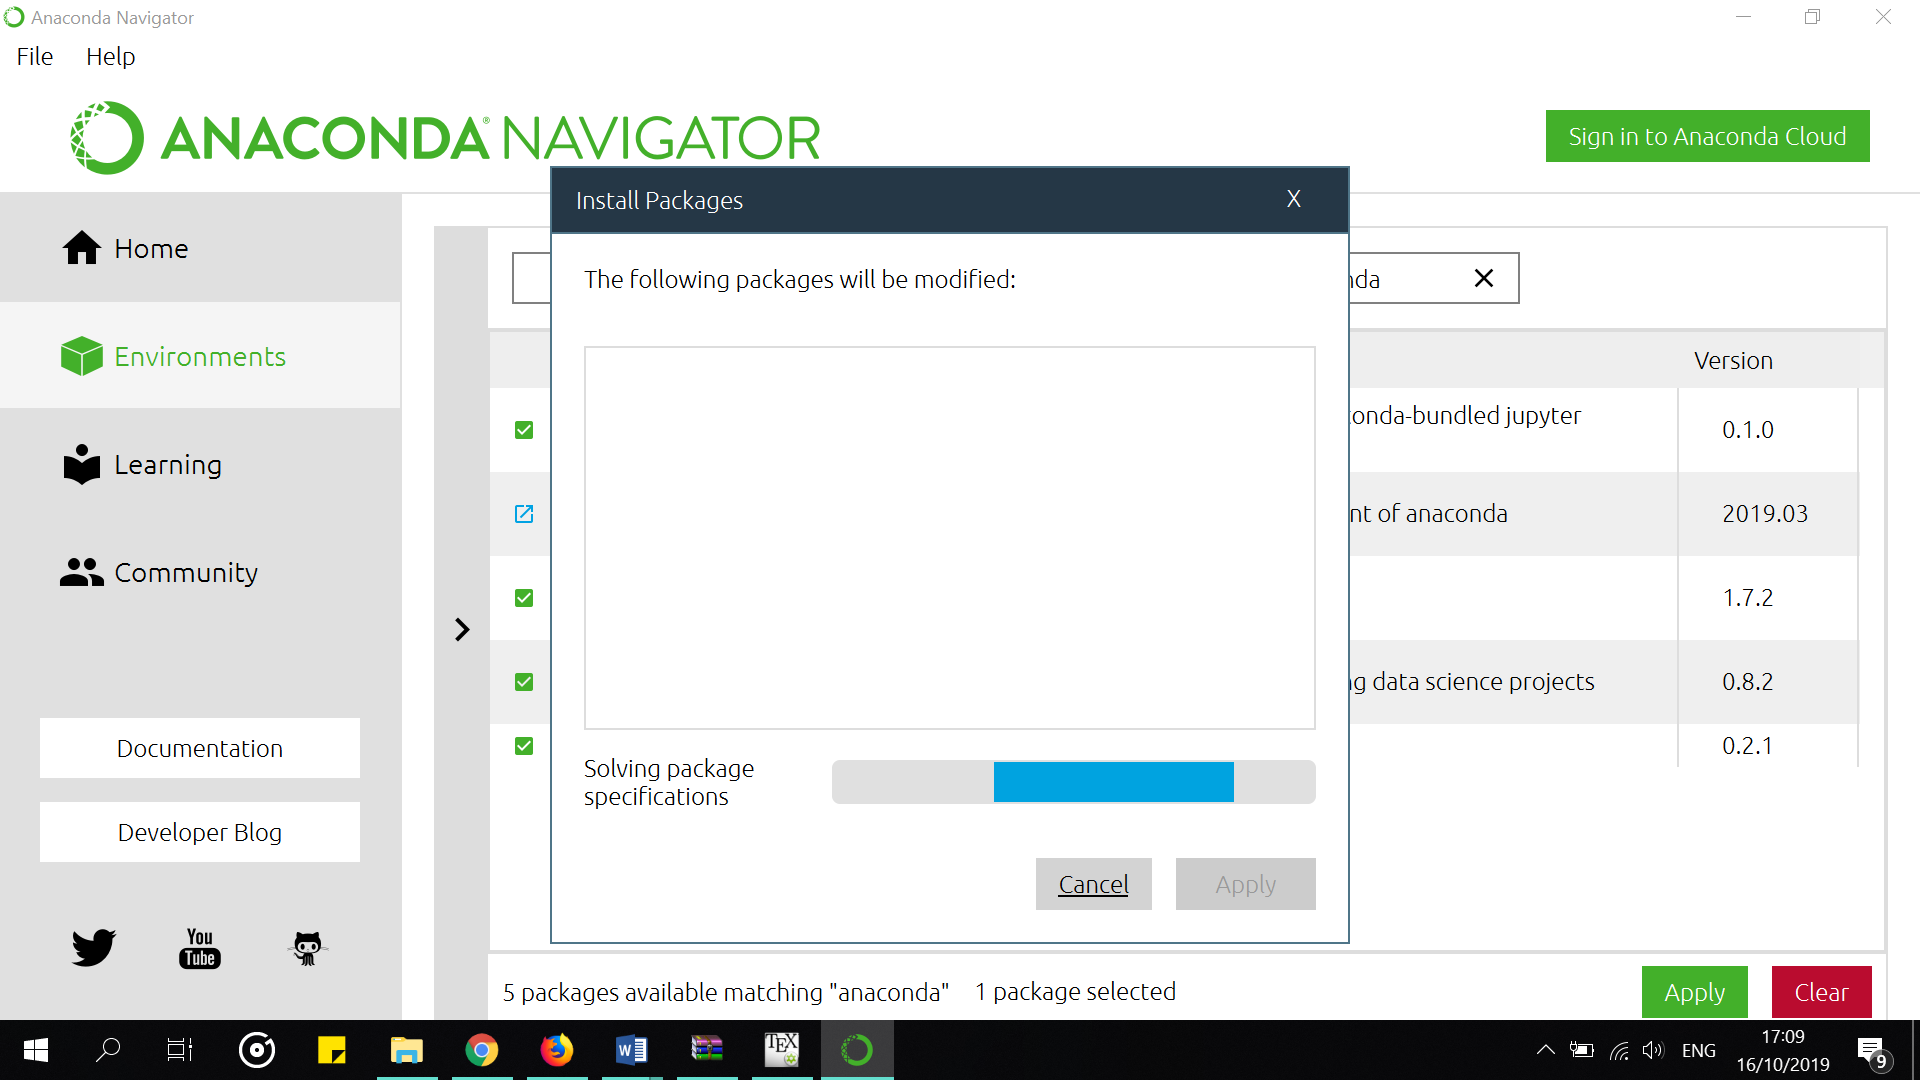
\includegraphics[width=10cm]{gambar/envi8.png}
\caption{environment}
\end{figure}
\item Klik Apply.
\begin{figure}[!htbp]
\centering
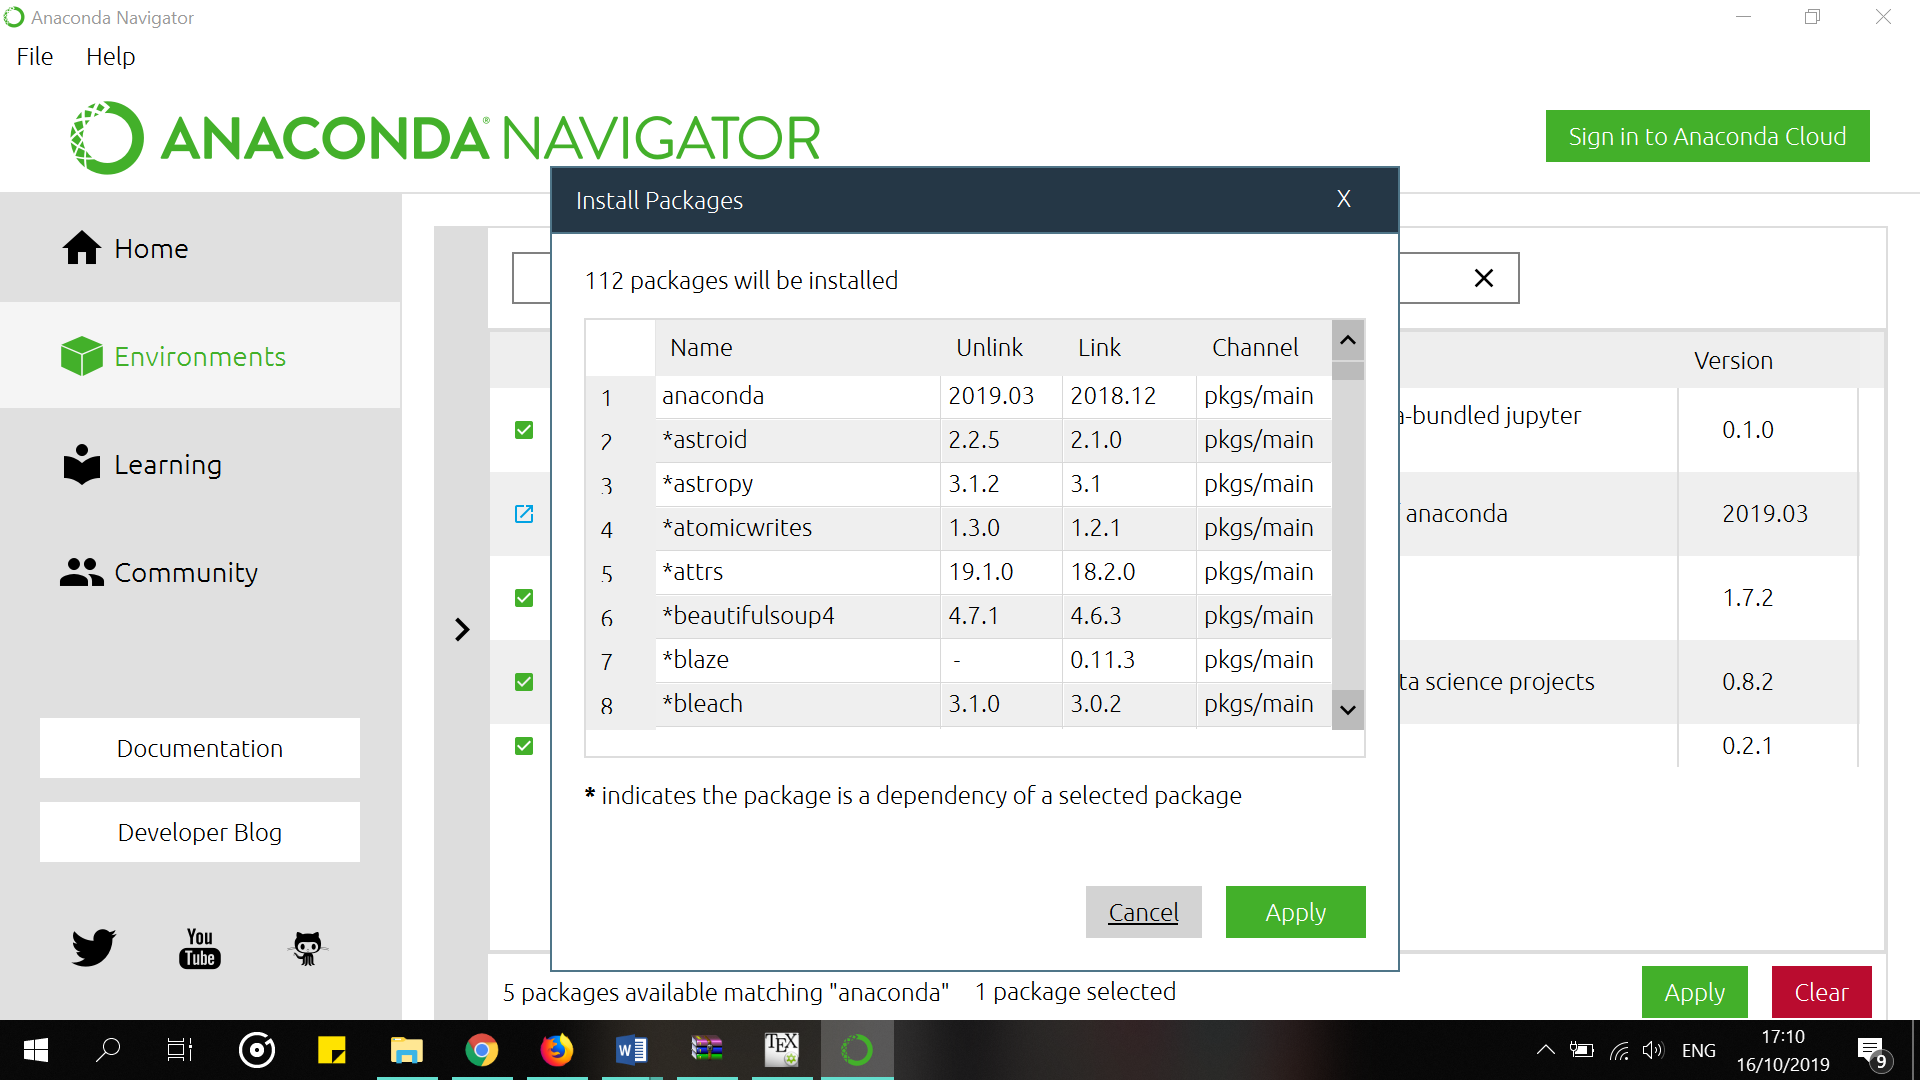
\includegraphics[width=10cm]{gambar/envi9.png}
\caption{environment}
\end{figure}
\item Tunggu sampai instalan selesai.
\end{itemize}
\item 	Menjalankan Anaconda dan Spyder
\begin{itemize}
\item Install Anaconda di https://www.anaconda.com/distribution/
\item Jika sudah didownload, buka installer Anaconda
\begin{figure}[!htbp]
\centering
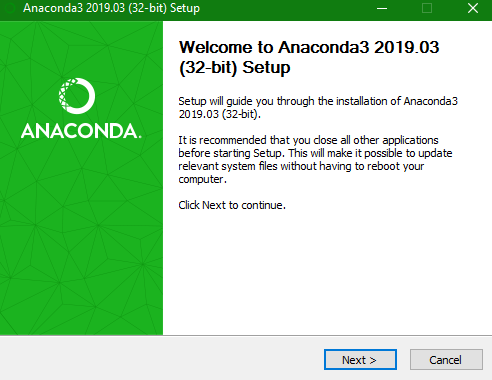
\includegraphics[width=10cm]{gambar/conda1.png}
\caption{install anaconda}
\end{figure}
\item Klik Next.
\item Kemudian Pilih lokasi tempat penyimpanan aplikasi.
\begin{figure}[!htbp]
\centering
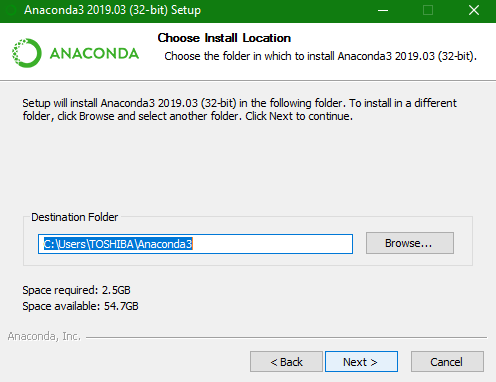
\includegraphics[width=10cm]{gambar/conda2.png}
\caption{install anaconda}
\end{figure}
\item Lalu pilih Just Me(recommended) agar sesuai dengan computer yang anda miliki.
\begin{figure}[!htbp]
\centering
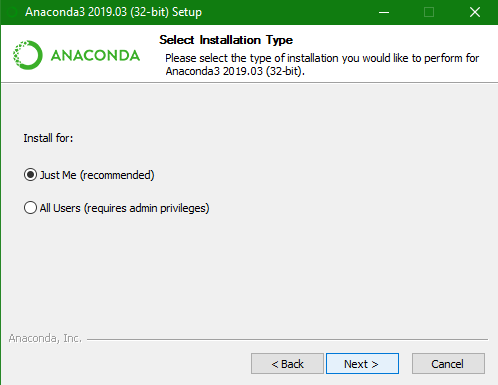
\includegraphics[width=10cm]{gambar/conda3.png}
\caption{install anaconda}
\end{figure}
\item Klik Next.
\item Kemudian ceklis Add Anaconda to my PATH.
\begin{figure}[!htbp]
\centering
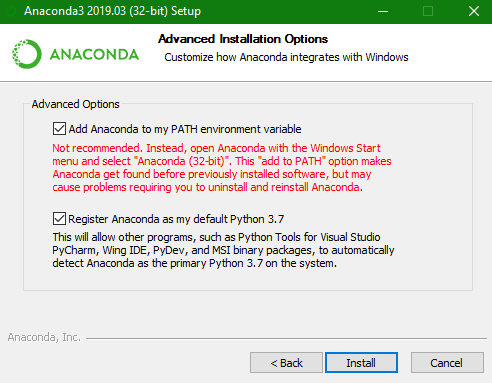
\includegraphics[width=10cm]{gambar/conda4.png}
\caption{install anaconda}
\end{figure}
\item Lalu anda centang Add Anaconda to my Path environment variable, agar saat mengisntall selenium langsung ke path anaconda tidak ke aplikasi yang lain.
\item Jika sudah klik install, tunggu sampai selesai proses installasi selesai.
\begin{figure}[!htbp]
\centering
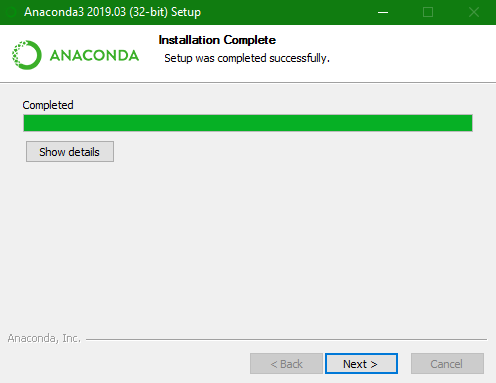
\includegraphics[width=10cm]{gambar/conda5.png}
\caption{install anaconda}
\end{figure}
\item Klik Next.
\newpage
\begin{figure}[!htbp]
\centering
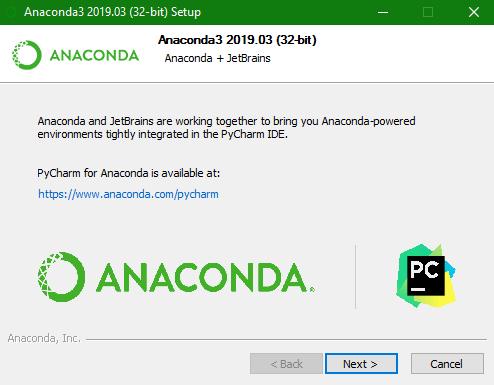
\includegraphics[width=10cm]{gambar/conda6.png}
\caption{install anaconda}
\end{figure}
\item Klik Next.
\begin{figure}[!htbp]
\centering
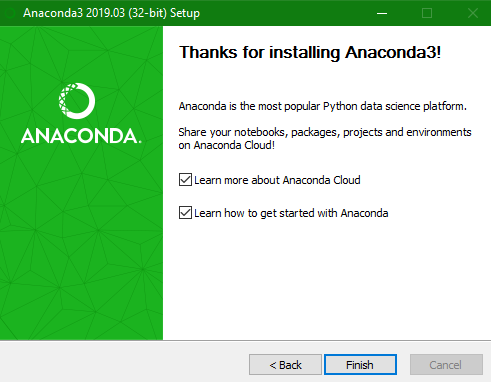
\includegraphics[width=10cm]{gambar/conda7.png}
\caption{install anaconda}
\end{figure}
\item Jika sudah klik Finish
\end{itemize}
\item Install Syder
\begin{itemize}
\item Buka Anaconda Navigator.
\item Lalu scrool ke bawah untuk menemukan spyder.
\begin{figure}[!htbp]
\centering
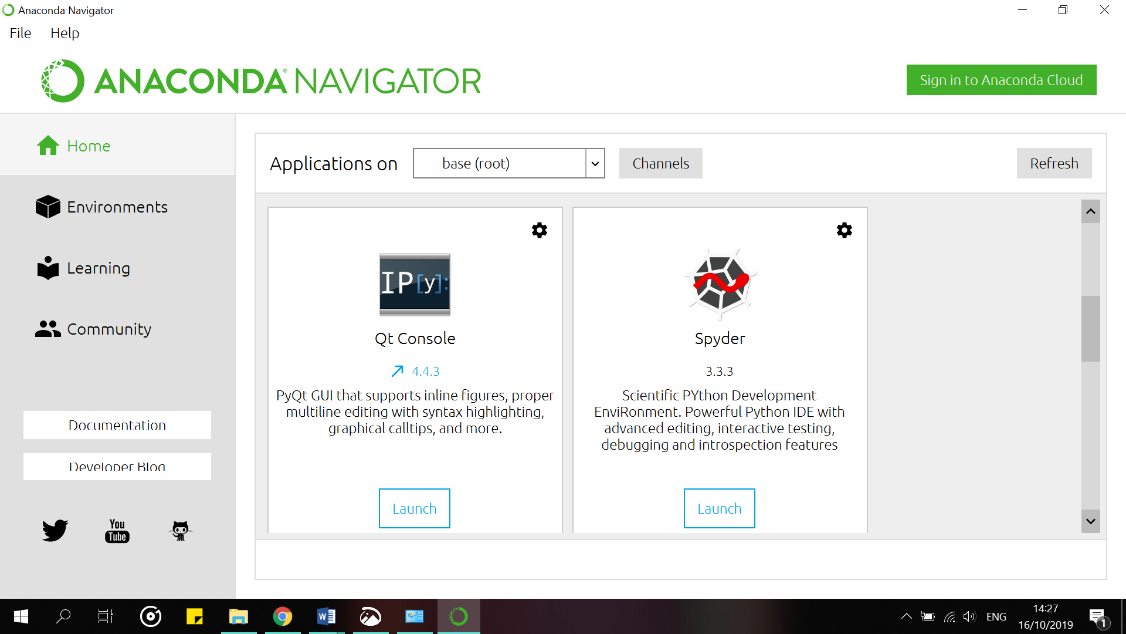
\includegraphics[width=10cm]{gambar/spy1.png}
\caption{install spyder}
\end{figure}
\item Lalu akan ada Spyder pada Anaconda Navigator
\item Lalu lunch spyder, maka spyder akan terinstal  otomatis.
\item Buka Spyder yang sudah di instal.
\begin{figure}[!htbp]
\centering
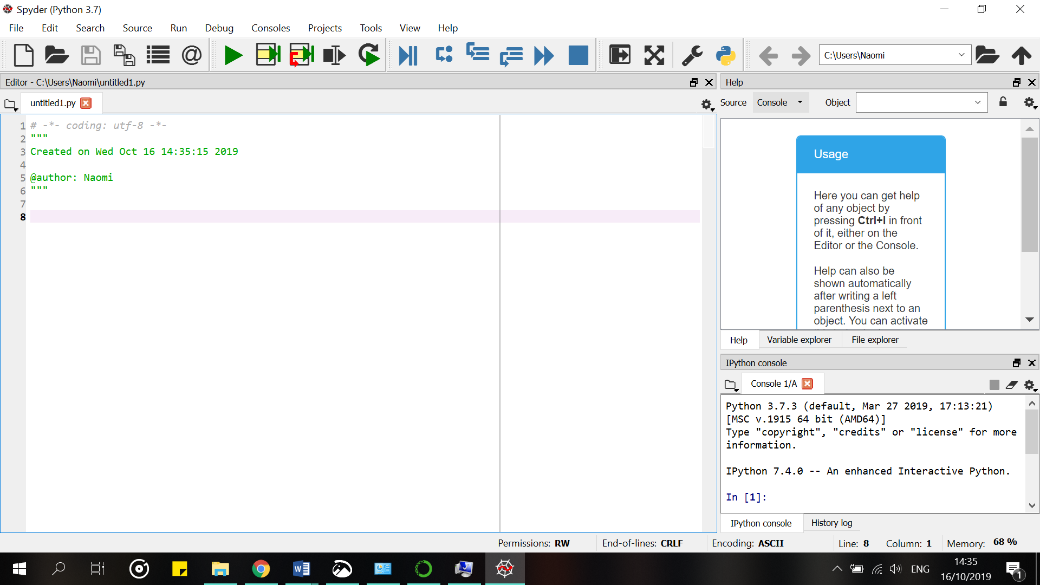
\includegraphics[width=10cm]{gambar/spy2.png}
\caption{install spyder}
\end{figure}
\end{itemize}
\item Cara Menjalankan Script Otomatis Login Akademik
\begin{itemize}
\item Buka spyder yang sudah di install.
\begin{figure}[!htbp]
\centering
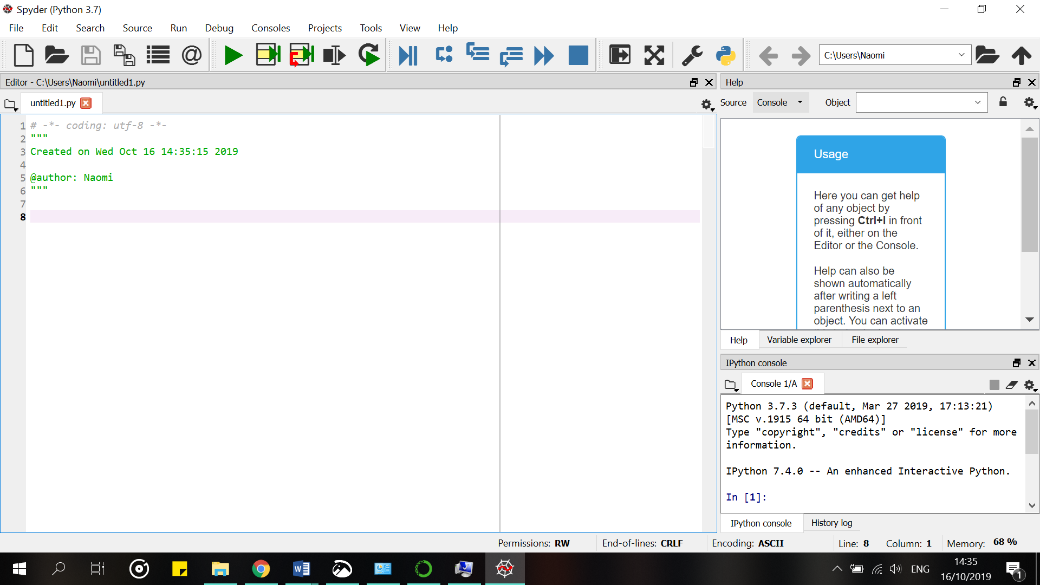
\includegraphics[width=10cm]{gambar/spy2.png}
\caption{spyder}
\end{figure}
\item Kemudian ketik codingan sebagai berikut agar bisa login ke browser akademik yang kita tuju.
\begin{figure}[!htbp]
\centering
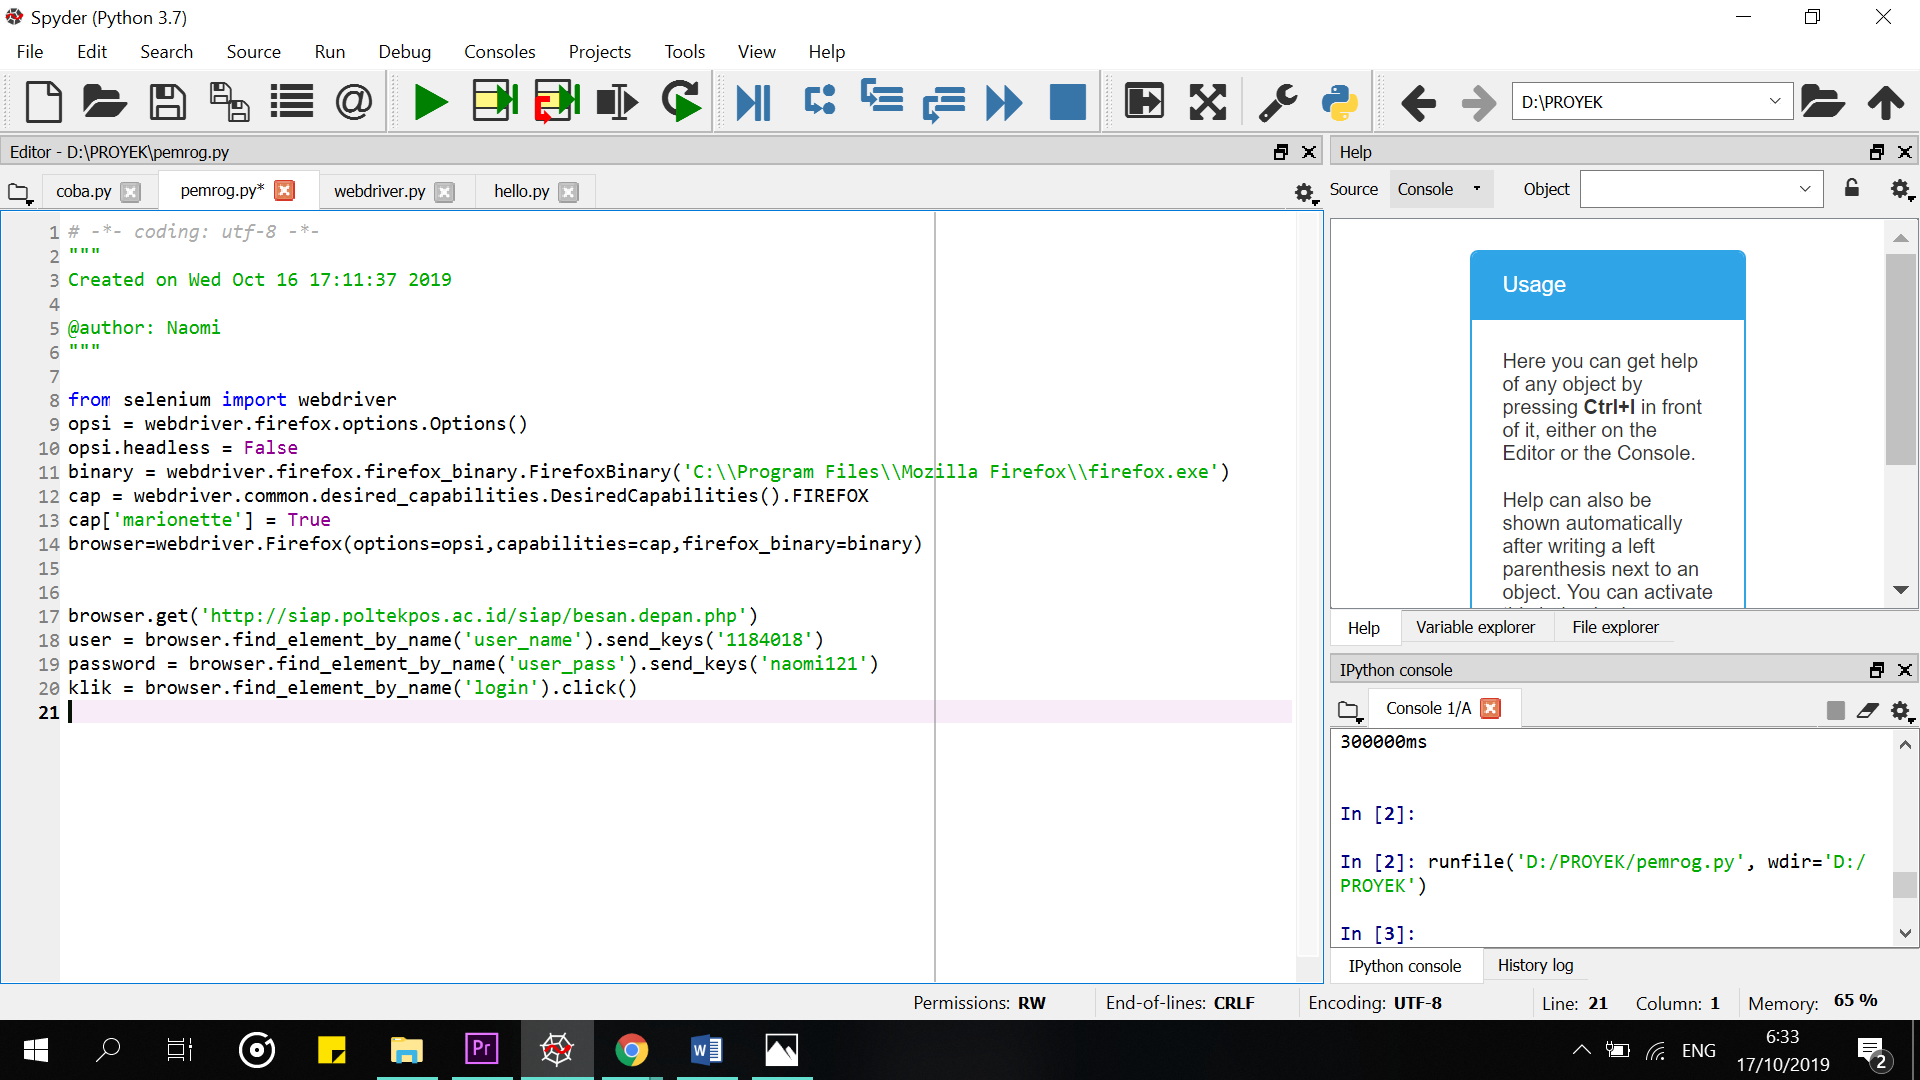
\includegraphics[width=10cm]{gambar/spy3.png}
\caption{spyder}
\end{figure}
\item Run Codingan yang telah diketik.
\begin{figure}[!htbp]
\centering
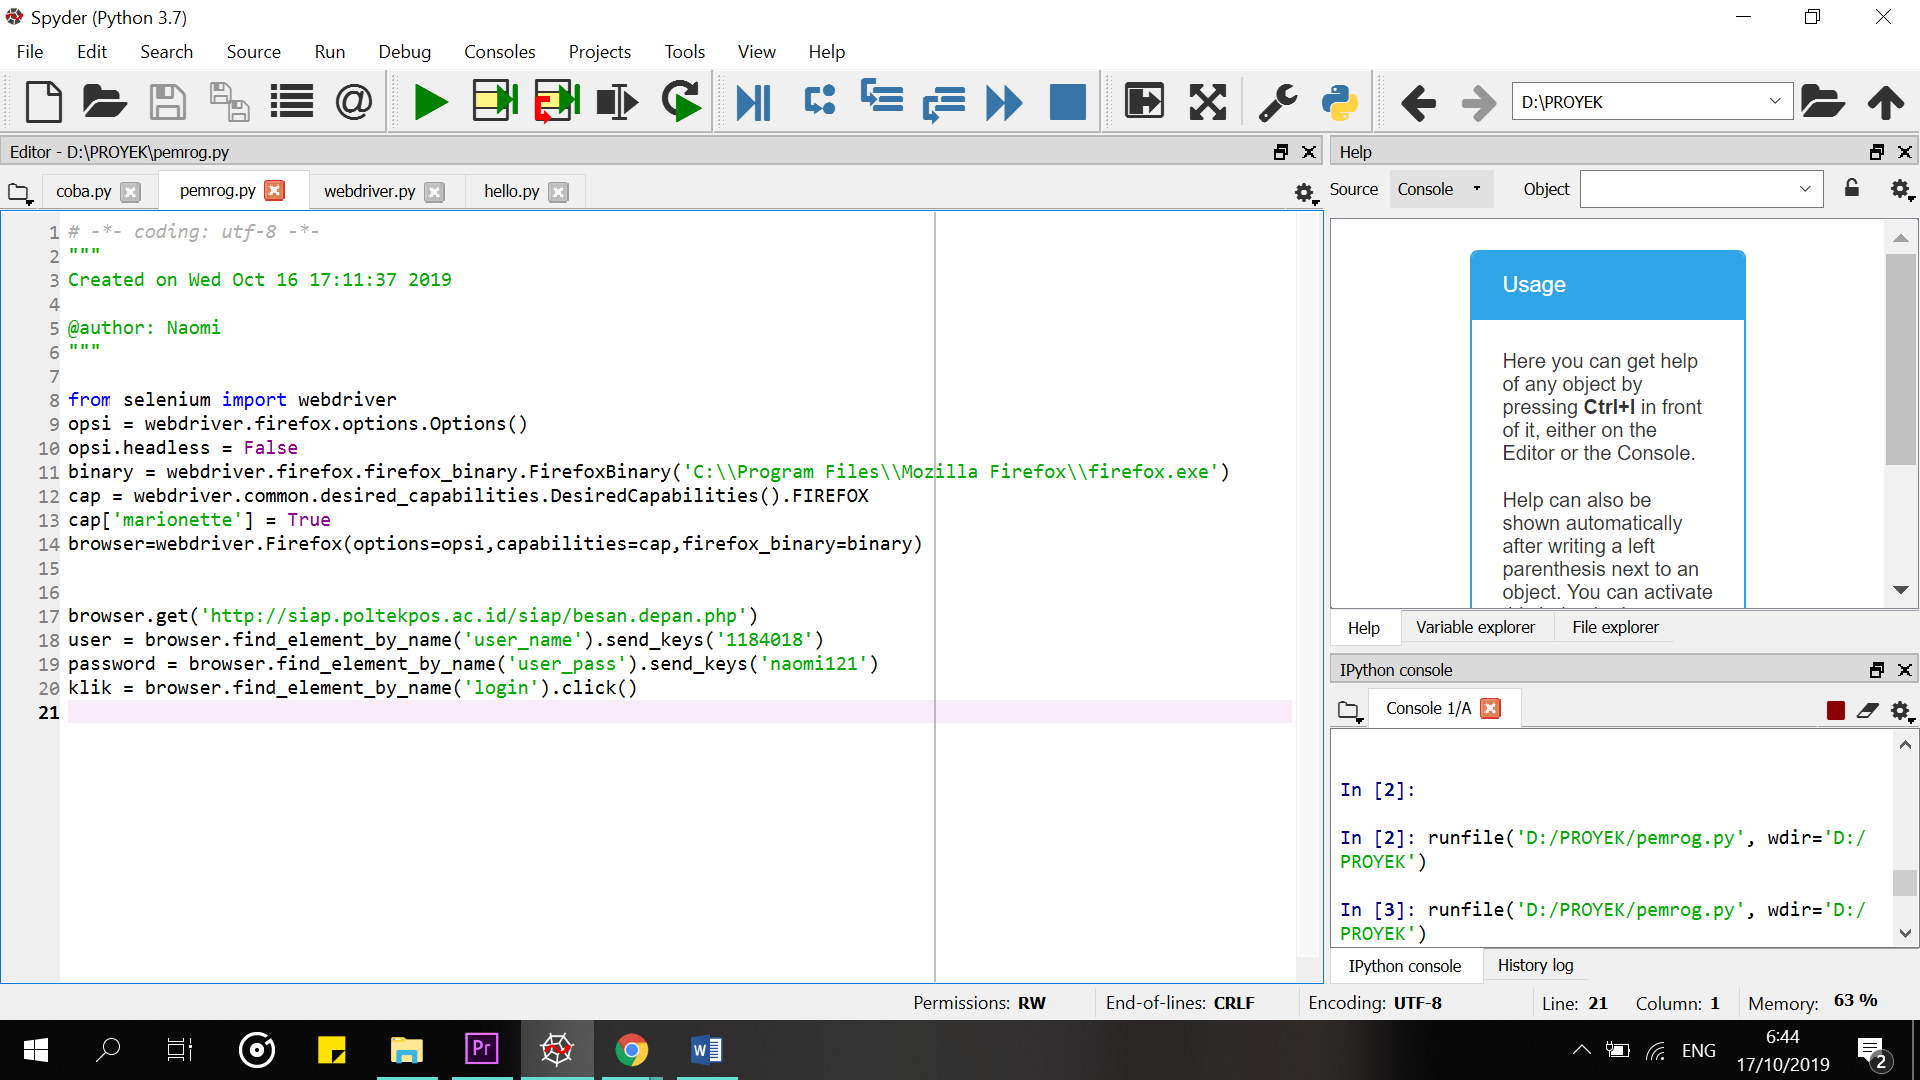
\includegraphics[width=10cm]{gambar/spy4.png}
\caption{spyder}
\end{figure}
\item Maka secara otomatis website siap.poltekpos.ac.id akan terbuka secara otomatis.
\begin{figure}[!htbp]
\centering
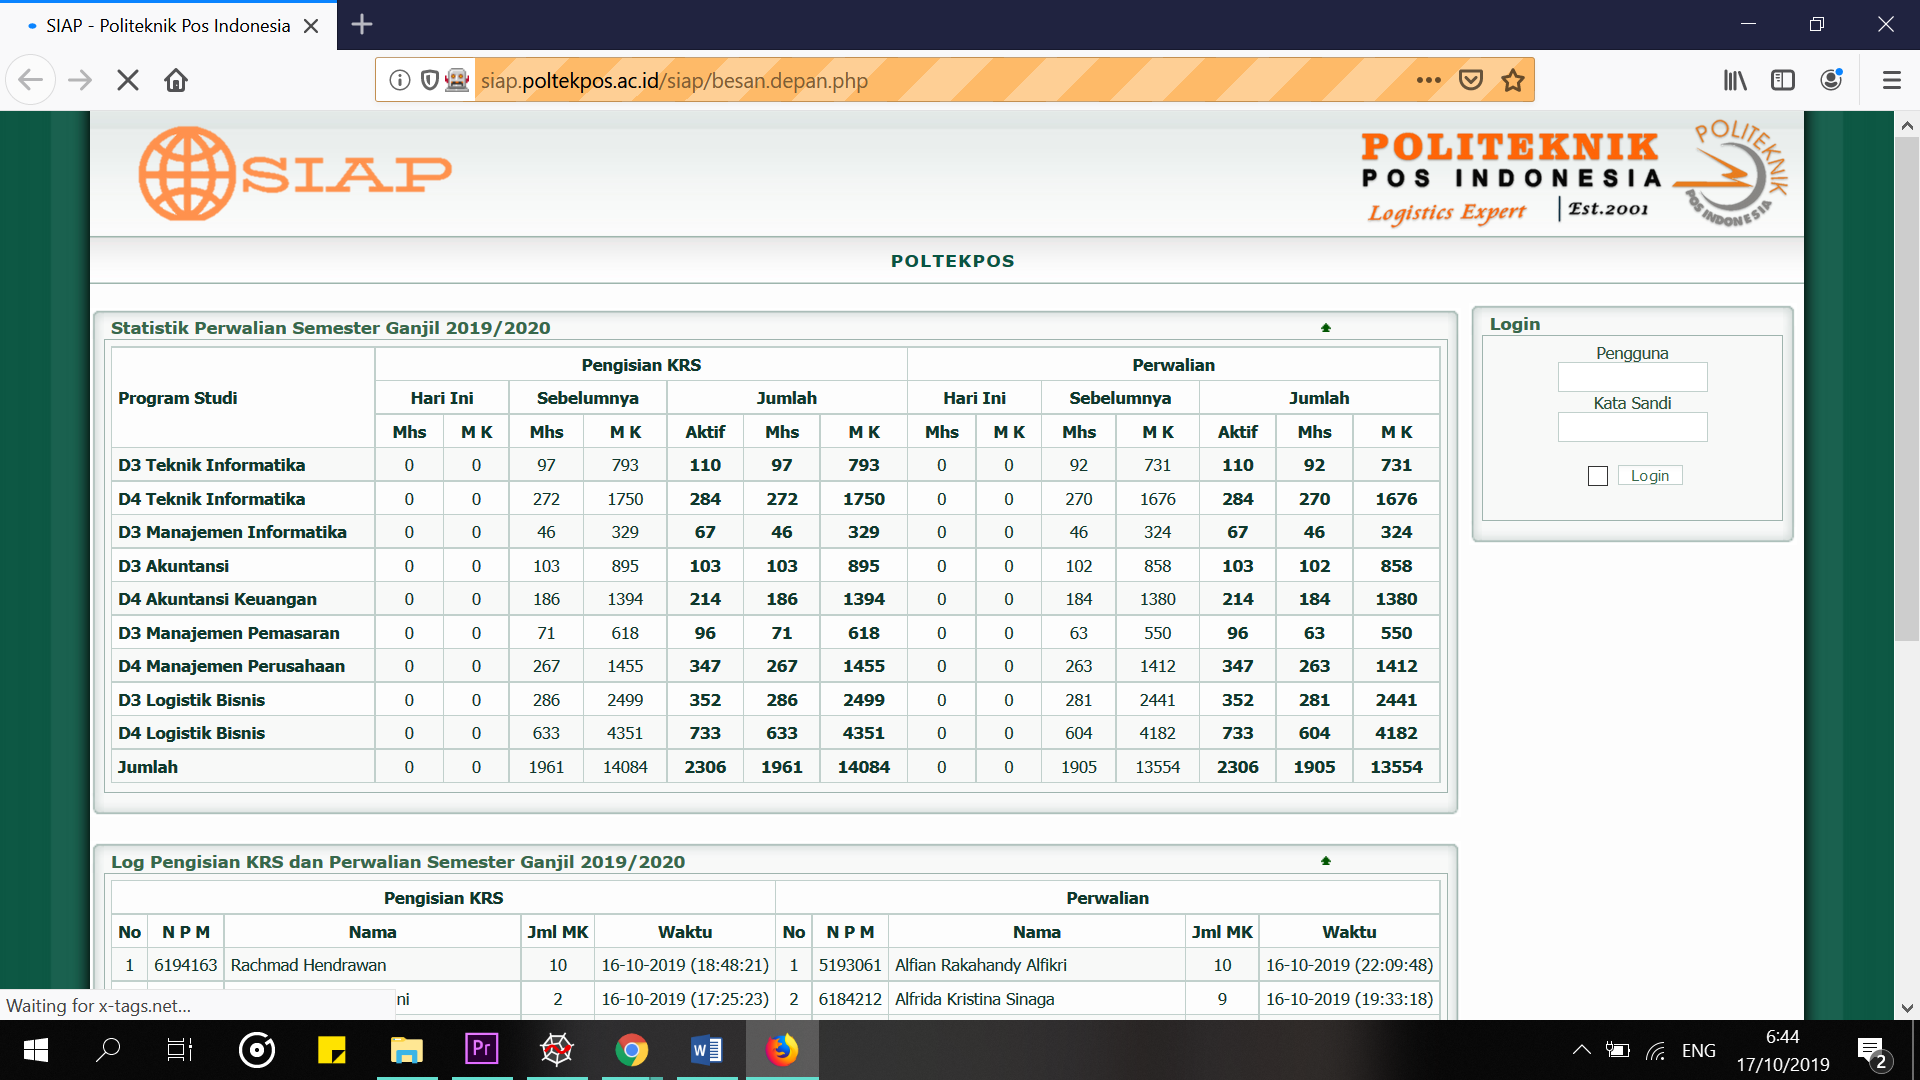
\includegraphics[width=10cm]{gambar/spy5.png}
\caption{spyder}
\end{figure}
\begin{figure}[!htbp]
\centering
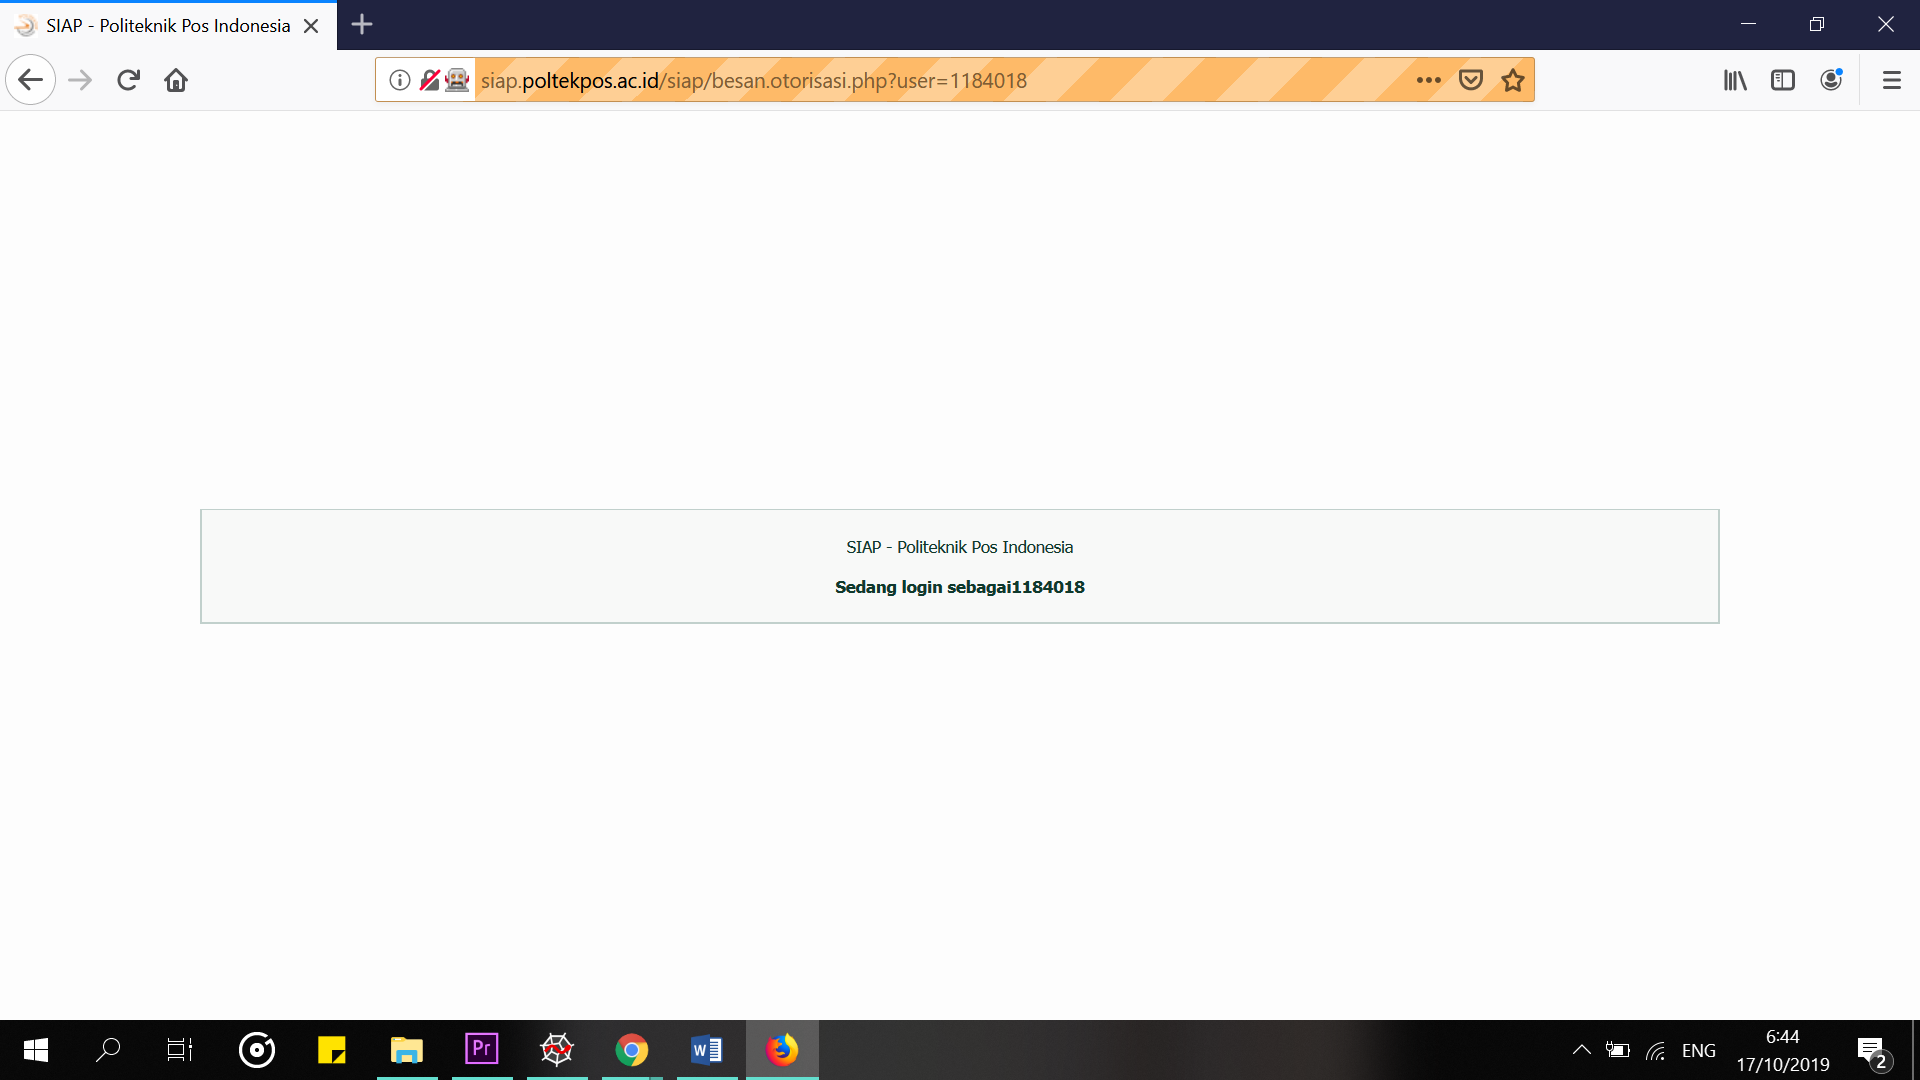
\includegraphics[width=10cm]{gambar/spy6.png}
\caption{spyder}
\end{figure}
\begin{figure}[!htbp]
\centering
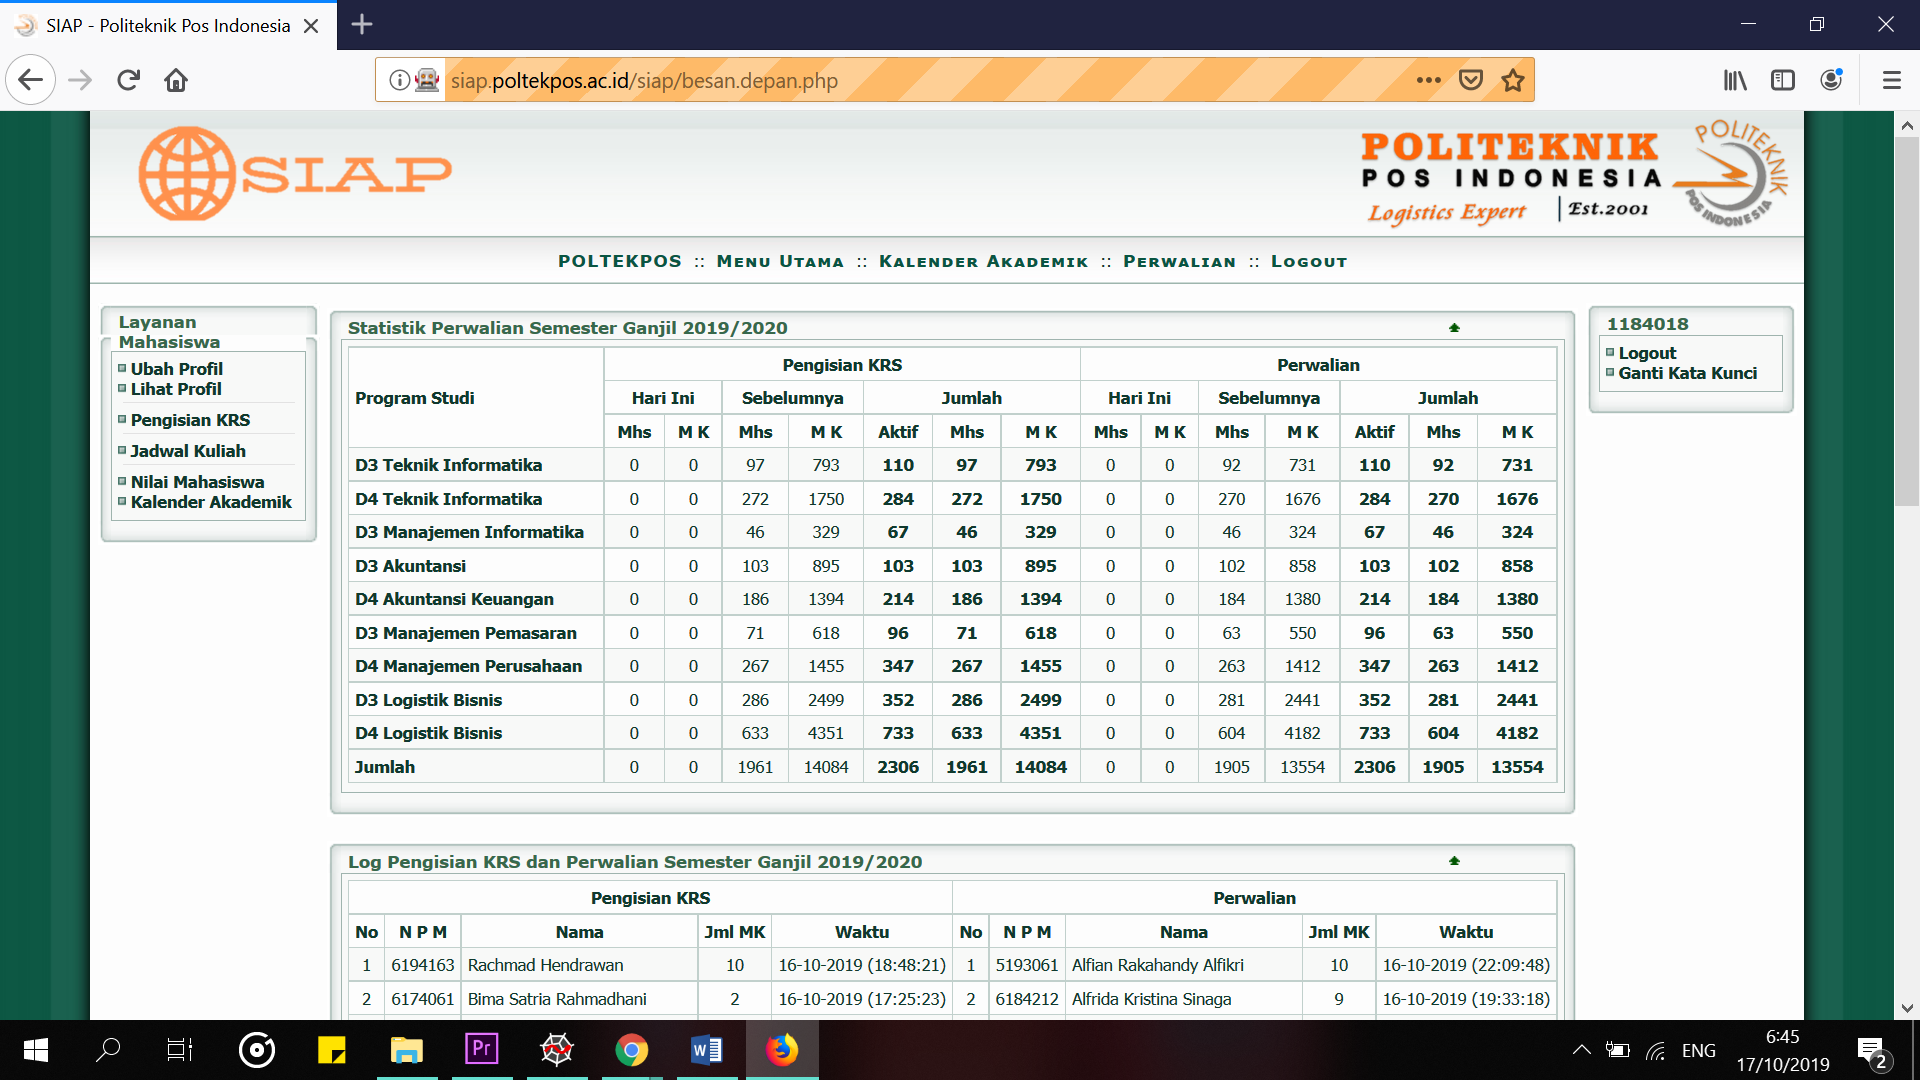
\includegraphics[width=10cm]{gambar/spy7.png}
\caption{spyder}
\end{figure}
\end{itemize}
\end{enumerate}